\documentclass[11pt,twocolumn]{article}

%\usepackage{sectsty}
\usepackage{titlesec}
\usepackage{url}

\usepackage{amssymb}

\usepackage{titlesec}

\usepackage{transparent}

\usepackage{setspace}
%\doublespacing
%\onehalfspacing

\usepackage{graphicx}
%\graphicspath{ {/ext_root/openshift-oc3/mmui-caf-local/web/mmui/public/pics/} }

\newcommand{\sectionGraphics}{

\vspace{2em}\centerline{\includegraphics[scale=0.125]{logo-deco.png}}\vspace{-1em}}

\usepackage[flushmargin]{footmisc}

\setlength{\parindent}{30pt}

%\usepackage{bigfoot}

%\DeclareNewFootnote[para]{R}[Roman]
%\DeclareNewFootnote[para]{N}

%\usepackage[letterpaper, left=1.3in,right=1in,top=1in,bottom=1in]{geometry}

\newcommand{\descItem}[1]{\item[{\color{logoRed!80!logoBlue}{\fontfamily{phv}%
\fontshape{it}\fontseries{b}\selectfont\scriptsize #1}}]}
%\newcommand{\descItem}[1]{\item[#1]}

\newcommand{\descItemLarge}[1]{\item[{\color{logoRed!80!logoBlue}{\fontfamily{phv}%
\fontshape{it}\fontseries{b}\selectfont\small #1}}]}


\usepackage{enumitem}

\setlist[description]{%
  topsep=30pt,               % space before start / after end of list
  itemsep=5pt,               % space between items
  font={\bfseries\sffamily}, % set the label font
%  font={\bfseries\sffamily\color{red}}, % if colour is needed
}


\usepackage{etoolbox}

\usepackage{mathptmx}
%\usepackage{euler}
%\usepackage{amsmath}

%\usepackage[LGRgreek]{mathastext}

%\sectionfont{\fontsize{12}{15}\selectfont}
%\subsectionfont{\fontsize{11}{12}\selectfont}

\titleformat*{\subsection}{\small\bfseries}

\usepackage{eufrak}
\usepackage{wasysym}
\usepackage{textcomp}
\usepackage{amssymb}

\usepackage{microtype}


\usepackage{graphicx}

\usepackage{tikz}

\usetikzlibrary{decorations.pathmorphing}
\usetikzlibrary{positioning}
\usetikzlibrary{shapes,snakes}


\let\OldSection\section

\renewcommand\section[1]{
	\vspace{9pt}
	
	\scalebox{1.3}{\colorbox{logoPurple!50}{\hspace{1em}}}
				
	%\hspace{-1.1cm}{\protect\includegraphics[width=1cm]{e-logo.png}}	
	{\protect\transparent{0.3}{\colorbox{logoPeach!10!blue}{%
			\begin{minipage}{\linewidth}
				    \vspace{.5em}
				
	\protect\transparent{1}{\OldSection{#1%
		%{\transparent{0.5}{
		%	\protect\includegraphics[width=1cm]{e-logo.png}
		%}
	    %}
     }}
	    \end{minipage}}} }
    
    \vspace{-5em}
    	{\protect\transparent{0.3}{\colorbox{logoPeach}{%
    		\begin{minipage}{\linewidth}
    			\hspace{\linewidth}
    	\end{minipage}}} } 
    
    \vspace{5em}
    
	\vspace{-6pt}
}

%\subsectionfont{\Large}
%\subsectionfont{\fontsize{12}{15}\selectfont}

\titleformat*{\subsection}{\Large\bfseries}

\let\OldSubsection\subsection
\renewcommand\subsection[1]{

	\vspace{12pt}
	
    %{\LARGE
	%\colorbox{logoCyan}{%
	%\begin{minipage}{\linewidth}
		\OldSubsection{% 	
			\hspace{-2.75em}
			%\begin{minipage}{}
			\protect\raisebox{-5pt}{%
			\colorbox{logoCyan!50}{\hspace{2.1em}}}%
			\hspace{-5pt}{\protect\transparent{0.3}{\colorbox{logoBlue!80}{\protect\transparent{1}{%
						   \protect\raisebox{1pt}{\textit{{\large #1}}} }}}}
			%\end{minipage}
		}
	%\end{minipage}
    %}
    %}
	\vspace{-6pt}
}



\newcommand*{\MyCircle}{\begin{tikzpicture}{baseline}
	\node [draw, shape=regular polygon, regular polygon sides = 5, shape border rotate=180,
	line width=.2mm, left color=blGreen, right color=darkBlGreen, draw=darkRed, aspect=1,
	draw opacity=0.6, fill opacity=0.8, xscale=0.5, yscale=0.5,
	minimum width=1mm, 
	] 
	at (0, 0) {};
	\end{tikzpicture}}


\newcommand*{\MyLabel}{%
 %\MyBall	
 %{\tikz \draw [baseline, ball color=red, draw=red] circle (3pt);} 	
 \protect\MyCircle{\hspace{4pt}}\color{flColor}\LARGE{\textbf{\protect\raisebox{-3pt}{\theenumi}}}
}

%
\newenvironment{colorDescription}{%
\vspace{1em}\begin{description}[style=nextline]}{\end{description}}

\newcommand*{\MyDiamond}{%
	\begin{tikzpicture}{baseline}
	
	\node [draw, shape=diamond, %shape border rotate=100,
	line width=.2mm, left color=flColor, right color=darkRed, draw=logoPurple, aspect=1,
	draw opacity=0.6, fill opacity=0.8, xscale=0.5, yscale=0.5,
	minimum width=1mm, 
	] 
	at (2, 0) {};
	
	\end{tikzpicture}
	
} 

\usepackage{enumitem}

\newcommand*{\MyDiamon}{*} 


\newenvironment{colorItemize}{\vspace{1em}\begin{itemize}[label={\MyDiamond}]}{\end{itemize}}

\newenvironment{colorEnumerate}{\vspace{1em}\begin{enumerate}[label=\MyLabel]}{\end{enumerate}}

\newcommand{\PeoplesVoiceCafe}{{\relscale{0.8}{\fontfamily{fvs}\fontseries{b}\selectfont%
 Peoples' Voice Cafe}}}
 
\newcommand{\q}[1]{{\fontfamily{qcr}\selectfont ``}#1{\fontfamily{qcr}\selectfont ''}} 

\usepackage{tcolorbox}

%\usepackage[framemethod=TikZ]{mdframed}

%
\tcbuselibrary{skins}
%\tcbuselibrary{listings,breakable}
\usetikzlibrary{calc}
\usetikzlibrary{shadows}
\pgfdeclarelayer{background}
\pgfdeclarelayer{foreground}
\pgfsetlayers{background,main,foreground}

\definecolor{BaseColor}{HTML}{8533FF}

\newlength{\boxShadowOfset}
\setlength{\boxShadowOfset}{2mm}

\newcommand{\tc}[1]{
\vspace*{-2.05cm}\hspace{1cm}
\begin{tcolorbox}
[colframe=cyan!10!black,boxrule=0.5pt,arc=8pt,hbox,enhanced, 
leftrule=5pt,rightrule=3pt,toprule=0pt,toprule=0pt,
%drop fuzzy shadow southeast={BaseColor!50!white},
%frame code={
%        },
     % left=6pt,right=6pt,top=6pt,bottom=6pt,
      boxsep=0pt]      
\protect{#1}
\end{tcolorbox}      
\vspace*{0.4cm}

}

\newcommand{\cursive}[2]{{\LARGE%
%\begin{minipage}{0.5\textwidth}
\protect\tc{%
%\protect\fcolorbox{cyan!10!black}{white}{
\protect\raisebox{-2pt}{
{\color{logoBlue!90!cyan}{%
{\fontfamily{bch}\fontseries{b}\selectfont%
 \larger{#1}}}}}{{\color{logoBlue!90!cyan}{\Fontlukas\bfseries\textsc{#2}}}}%
%\end{minipage}
%}
}}}
%\end{minipage}

\newcommand{\parlead}[1]{\vspace{1.15em}\noindent{%
{\color{logoRed!80!logoBlue}{\fontfamily{bch}\fontseries{b}\selectfont\large #1}}}}

\newcommand{\itemLarger}[1]{\item {\raisebox{-2pt}{\larger{#1}}}}

\newcommand{\itemLargerLine}[2]{\item {\raisebox{-2pt}{\larger{#1}}}%
\hspace{1em}{\raisebox{-2pt}{#2}}}

\newcommand{\p}{

\vspace{.45em}}

\newcommand{\txtbl}{\hspace{2pt}{{\raisebox{1pt}{\relsize{-2}\textbullet}}}\hspace{2pt}}

\newcommand{\colorhref}[1]{\colorbox{blGreen!20}{#1}}



\PassOptionsToPackage{svgnames}{xcolor}

\usepackage[object=vectorian]{pgfornament} %%  http://altermundus.com/pages/tkz/ornament/index.html
\usepackage{lipsum,tikz}

\newcommand{\sectionline}[1]{%
  \noindent
  \begin{center}
  {\color{#1}
    \resizebox{0.5\linewidth}{1ex}
    {{%
    {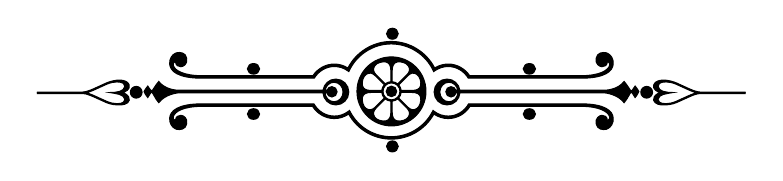
\begin{tikzpicture}
    \node  (C) at (0,0) {};
    \node (D) at (9,0) {};
    \path (C) to [ornament=84] (D);
    \end{tikzpicture}}}}}%
    \end{center}
  }
%% A macro with two arguments to change ornaments and colors easily
%% Syntax -- \sectionlinetwo{<color>}{<ornament>}
\newcommand{\sectionlinetwo}[2]{%
  \nointerlineskip \vspace{.5\baselineskip}\hspace{\fill}
  {\color{#1}
    \resizebox{0.5\linewidth}{2ex}
    {{%
    {\begin{tikzpicture}
    \node  (C) at (0,0) {};
    \node (D) at (9,0) {};
    \path (C) to [ornament=#2] (D);
    \end{tikzpicture}}}}}%
    \hspace{\fill}
    \par\nointerlineskip \vspace{.5\baselineskip}
  }

\newcommand{\EnglischeLinie}{
\sectionline{darkRed!60!cyan}
}

\newcommand{\lMOSAIC}{\mbox{MOSAIC}}
\newcommand{\lfMOSAIC}{\mbox{M\small{OSAIC}}}
\newcommand{\MOSAIC}{\mbox{\small{MOSAIC}}}
\newcommand{\RAK}{\mbox{\small{RAK}}}
\newcommand{\SDK}{\mbox{\small{SDK}}}
\newcommand{\lSDK}{\mbox{SDK}}
\newcommand{\GUI}{\mbox{\small{GUI}}}
\newcommand{\qvspace}{\vspace{.4em}}
\AddToShipoutPicture{%
  \AtPageLowerLeft{%
    \hspace*{1em}
 \rotatebox{90}{%
        \begin{minipage}{\paperheight}
   \centering
   {\color{codegr!65}\textcopyright ~\today{} Nathaniel Christen}
        \end{minipage} %
      }
    } %
  }%
\begin{document}\title{NASM}
\maketitle{}
\begin{abstract}NASM
\end{abstract}
\begin{quote}Now, the \q{science of salience}
proposed by Petitot and Smith (1997) illustrates the
kind of formalized analysis made possible through the direct
mathematization of phenomenological descriptions.
Its aim is to account for the invariant descriptive
structures of lived experience (what Husserl called \q{essences})
through formalization, providing a descriptive geometry of
macroscopic phenomena, a \q{morphological eidetics} of the
disclosure of objects in conscious experience (in Husserl's
words, the \q{constitution} of objects).
Petitot employs differential geometry and morphodynamics
to model phenomenal experience, and Smith uses formal structures from
mereotopology (the theory of parts, wholes, and their boundaries)
to a similar effect.
\end{quote}  \mdash{}  Maxwell James Ramstead
\vspace{1em}
\p{Computational and scientific data representation intrinsically 
balances two competing priorities: \q{semantic} expressiveness and 
computational tractability.  On the one hand, representations should not 
obscure important details: the formal requirements on 
representational validity should not force representations 
into structures that necessitate the elimination of meaningful 
information.  On the other hand, conversely, representations 
should have enough structural consistency that they are 
amenable to analysis and transformations driven by 
formal algorithms.
}
\p{I have just left a lot of loose ends: in particular, these comments need 
to give some meaningful definition to \q{representation}.  There 
are many media wherein \q{data} can be represented: via graphics 
(e.g., charts, \q{maps} in the cartographical sense, or \q{graphs} 
in the sense of plotted visualizations of 
mathematical functions), via printed documents (like the logarithmic 
tables or astronomic records of early modern science), or via mathematical 
equations and formulae (if a mathematical theory correctly 
predicts and quantifies empirical data \mdash{} e.g., fitting trajectories 
to elliptic or parabolic shapes \mdash{} then the numeric structures of 
the theory are a proxy representation of the corresponding data).  
Moreover, aside from these relatively formal modes of representation, 
we have the capacity to indirectly describe information via 
natural language. 
}
\p{The modern age has a further notion of representation: \i{digital} 
representations which leverage the capabilities of 
computer storage and processing to create persistent 
data repositories, with the possibility of manipulating 
data via computer programming and displaying data 
via computer software.  These digital representations incorporate 
features of the older representational media I alluded to: 
like Natural Language digital data often emanates from a 
textual representation, with data structures initialized 
from special \q{languages} like \XML{} or \JSON{}.  As with 
structured \q{printed} documents (of the astronomical-table 
or even grocery-shopping-list variety), digital representations 
often build off of a rigid structural template, like a two-dimensional 
table with rows and columns, or a hierarchical document 
whose elements can be nested documents.  And as with 
mathematical representations, digital representations can be 
analyzed as instances of spaces or structures with certain 
algebraic or syntactic properties and requirements.  
It is often possible to mathematically describe the 
full space of structures which conform to a given 
representational protocol, or the full space of transformations 
that can modify a given data structure while staying 
consistent with its enforced protocols.  Also, each data 
structure potentially has some notion of aggregateness: of 
having different \q{parts}, of being able to focus on one part 
at a time, and to \q{move} focus from one part to another.  
Given these qualities, digital representations extend and integrate  
the affordances of print, graphical, and linguistic media 
\mdash{} but they do so in an electronic environment that permits digital 
archives to be accessed via computer software.  With sotfware as their  
access point, digital representations can inherit the formal properties of 
the software that uses them, so we can think of digital representations as 
formal structures themselves, amenable to something like a mathematical analysis. 
}
\p{In short, digital representations have several general criteria: 
\i{validity} (a formal model of conformant vs. invalid 
structures\footnote{An invalid graph might be a case where an 
edge has no incident nodes; an invalid \XML{} structure is one without 
a single root element or (insofar as such a structure would be 
representable) with mismatched tags, and so forth)}); 
\i{traversability} (a notion of parthood and iterating
or refocusing among parts), and, let's say, \i{atomicity} 
(a notion of unitary parts that can be represented as 
integral wholes).  These criteria ensure that digitally 
represented data structures can work within software and 
networking representations: information is 
presented to software users by displaying atomic 
units (textually or graphically) and traversing through 
data structures to fill in, via application code, a 
visual tableau presenting compound data, with different 
unitary displays visually separated and often organized into 
coherent visual patterns, like the grid-pattern of a 
spreadsheet.  Meanwhile, atomic units can be textually 
encoded, and aggregate structure likewise notated through 
syntactic conventions that preserve atoms' boundaries, yielding 
textual serializations of data structures that can be 
shared between computing environments, allowing information to 
be copied and distributed.  Finally, digital representations 
of data structures can be marshalled into different binary forms \mdash{} 
encoded in byte- and bit-patterns \mdash{} to enable both 
persistent storage in a database and \q{runtime} presence 
as binary data that may be accessed by software applications.
}
\p{I take the time to lay out these basic principles because I want 
to emphasize the different contexts where digital representations can be 
found: in particular, textual encoding and serialization; 
graphical/interactive displays for software users; application runtimes; 
and long-term database storage.  A given representation will morph and 
mutate to accommodate these different contexts.  Moreover, these 
contexts correspond to distinct technical specializations: database engineers 
have a different perspective on data structures than network engineers designing 
protocols for encoding and exchanging data between network endpoints; and 
application designers focused on optimal human-computer-interaction 
understand digital representations as visual and interactive phenomena, 
whereas application \i{developers} need to focus on how to 
properly encode data structures for binary runtimes.  These various 
perspectives all influence the theory and technology 
behind digital data representation \mdash{} a successful 
representational paradigm needs to adapt to the operatoonal 
requirements of engineers in each of these disicplines.
}
\p{Additionally, insofar as the point of digital archives is to encode 
empirical, \q{real-world} data, a proper representational protocol 
needs to promote a synergy between the information as humans understand 
it and the data structures recognized by the technology.  For instance, 
if a published data set shares scientific data, it should be 
represented in ways that preserve scientifically significant 
details \mdash{} any derivations, descriptions, or observations 
which are intrinsic to the science's methodology, 
theory, assumptions, and experimental results.  The data needs to 
be structured according to the \q{semantics of the science}, so that 
the scientific background can be reconstructed along with future use 
of the data, even after a circuitous journey through different 
contexts, like through a database and over a network to 
a scientific-software application (maye years later).   
As formal models of data semantics have become more rigorous \mdash{} e.g. in our 
century with Ontologies and the \q{Semantic Web} \mdash{} this 
\q{semantic engineering} has become a further technical perspective 
needing consideration in the design and evaluation of digital representations.
}
\p{Over the decades, many digital representation strategies and 
\q{layouts} have been envisioned, from tabular structures 
in the manner of Relational Databases, to tree-like 
documents whose morphology is inspired by markup languages, 
to structurally looser variations on row/column 
arrangements like multi-dimensional key-value spaces or 
\q{Big Column} and other \q{\NoSQL{}}-database-inspired 
articulations.  These various paradigms are subject to 
selective pressures based on how well they meet the 
different engineering needs I have identified.  But the 
multiplicity of requirements complicates the \q{competition} between 
representational strategies: a paradigm optimized 
for one context (e.g., persistent databases) is not necessarily 
optimal for another (e.g., application and \GUI{} development).  
As a result, developers and computer scientists must 
continue to explore and collaborate on new paradigms which 
work better across contexts.
}
\p{In the plurality of representational paradigms, a significant 
evolution has been the emergent popularity of structures 
based on graphs.  The predominant influence on this 
line of development has been the Semantic Web and the specific graph 
architecture codified by \q{Web Ontologies}, although 
other graph-representation models (such as 
Conceptual Graph Semantics) were also candidates for 
potential technological \q{entrenchnment} before 
Semantic Web formats like \RDF{} and \OWL{} 
became standardized.\footnote{Why \RDF{}/\OWL{} and not, say, Conceptual 
Graphs, or the hybrid Object-Database/Graph-Database models 
studied in the 1990s, became canonized in the Semantic Web, is 
an interesting question but perhaps of mostly historical 
interest insofar as Hypergaphs can unify each of these paradigms.
}  More recently, scientists have proposed generalizations 
and/or alternatives to the Semantic Web based on 
hypergraphs in lieu of ordinary (directed, labeled) graphs.
}
\p{As might be ascertained from hypergraphs being the focus of this paper, 
I believe that representational paradigms based on hypergraphs can be superior to 
other formats and need to be studied with an integrated, generalized 
set of theories and computer tools.  I have introduced the 
topic of hypergraph data structures via general issues in 
digital representation in part to rest claims of hypergraphs' 
merit on explicit criteria.  In particular, I believe 
hypergraphs can adapt to the different technological 
contexts prerequisute to a decentralized digital ecosystem 
\mdash{} databases, networking, application implementation, visual/interactive 
software design, and semantic expressiveness \mdash{} more effeectively 
than other paradigms, like regular graphs or \SQL{}-style tables.
}
\p{I suspect other scientists and engineers have 
similar intuitions, because there has been a recent uptick in 
research on hypergraphs in various disciplines, such 
as Category Theory, Information Management, Artificial Intelligence, 
and Natural Language Processing.  Compared to 
the Semantic Web, however, there is a noticeable lack 
of standard tools or formats for expressing hypergraph 
data or sharing hypergraph structures across multiple 
applications and environments.  Whereas \RDF{} and \OWL{} are 
definitively associated with the Semantic Web, so that 
supporting these standards is a basic entry point for 
Semantic Web technologies, there is no comparable 
consensus on the underlying theory of hypergraph data 
in general.    
}
\p{This situation may be explained in part by subtle differences on 
what the word \q{hypergraph} is supposed to mean in different 
settings, so the overal terrain of hypergraphs is 
divided into distinct mathematical models, often without a 
rigorous theory of their interrelationships.  
Another problem is perhaps a failure to appreciate how hypergraphs 
are structurally different from ordinary graphs, so that 
hypergraph-shaped data may be imprecisely treated as 
a mere variation upon or a special structuration within 
ordinary graphs.  For eample, Semantic Web structures such as 
\RDF{} \q{bags} and \q{collections} introduce a kind of 
hierarchical organization to Semantic Web graphs \mdash{} qualifying as 
a form of hypergraph \mdash{} but these protocols are not described as 
enabling a transition from a networking framework based on 
directed labeled graphs to one based on hypergraphs.  Instead, 
hypergraphs become \i{de facto} embedded within ordinary graphs, 
exploiting the representational flexibility which also 
makes the Semantic Web suitable for spreadsheets, \XML{}, and 
other structures that are not graphs at a \i{prima facie} level.
The problem is that while hypergraphs can be \i{encoded} in 
ordinary graphs with a suitable labeling convention, 
their distinct structural advantages are lost as 
explicit architectural features once hypergraphs are 
\q{encoded} in conventional Semantic Web formats.
}
\p{As I will outine in the first section, there are at least some half-dozen 
different structures that may certainly be described as hypergraphs, generalizing 
various underlying graph models (or indeed, even if we restrict attention to 
labeled directed graphs).  Within this space of possibilities, 
recent computer-science-related) research into hypergraphs 
seems to emphasize two different topics: first, the 
representational potential for hypergraphs as a 
general morphology for encoding structured information-resources 
(so as a general tactic for data warehousing and modeling); and, second, the 
specific possibilities of using hypergraphs to model computer code and computational 
processes.  In the second subject-area, hypergraphs are studied 
as a medium for expressing details about computer algorithms as a 
way to reason about executable computer code as a structured system, and 
perhaps even to design execution engines (virtual machines to 
run computer code that is in a suitable representation).  This 
latter research sometimes appears to present a mathematical 
picture of hypergraphs as an abstract model 
of computing procedures and evaluations \mdash{} a kind of 
graph-based interpretation of the lambda calculus \mdash{} but 
sometimes is also marshaled into implemented execution 
environments, as in the OpenCog and lmnTal frameworks.
}
\p{My goal in this paper is to consider what a unified hypergraph 
paradigm can look like \mdash{} how the different strands which in their 
own way embody hypergraph structures can be woven together 
into a multi-purpose whole.  My emphasis is on computer implementations 
rather than mathematics \mdash{} that is, I will not present axioms 
or theorems formalizing different sorts of hypergraphs, though I 
ackowledge that such descriptions are possible.  Instead, my 
aim is to describe what might constitute a general software 
library or toolkit that can adapt to different hypergraph 
models and use-cases.  This paper is accompanied by a \q{data set} 
which involves a library (written in \Cpp{}) for creating and 
manipulating hypergraphs of different varieties, and also a 
\q{virtual machine} for modeling and realizing 
computatational procedures via hypergraph structures.  The 
point of the accompanying code is to 
demonstrate that a generalized hypergraph representation 
is possible, and that in addition to use-cases for modeling 
data structures such a representation can be used at the 
core of a virtual processor.  The code includes simple tests and 
\q{scripts} that can be executed via the provided virtual-machine 
code.
}
\p{Studying hypergraphs from a computational (and 
\q{implementational}) perspective \mdash{} not just as 
mathematical objects \mdash{} introduces useful details 
that can add depth to our overall understanding of 
hypergraphs.  For example, one question is how hypergraphs 
can be initialized \mdash{} how software systems can build up 
hypergraph structures, piece by piece.  This is related to the question of 
proper serialization formats for hypergraphs.  Given some 
specific hypergraph data aggregate \Hy{}, it is important to 
have a textual encoding where \Hy{} can be mapped to a 
character-string, shared as a document, and then reconstructed 
with the same hypergraph structure.  This raises the question of 
when and whether two hypergraphs are properly isomorphic 
\mdash{} such that serializing and then deserializing a 
hypergraph yields \q{the same} hypergraph \mdash{} and also the problem 
of validating and parsing textual representations of hypergraphs.  
The theory of parsing \i{serializations} of hypergraphs \mdash{} 
textual encodings constructed according to a protocol wherein their 
grammar and morphology are suitable to 
expressing and then rebuilding hypergraph structures \mdash{} 
then becomes an extension of hypergraph theory itself.
}
\p{In addition to creating hypergraphs via textual 
representations in the manner of markup languages 
(like \XML{} or \RDF{}), we can also consider the incremental 
accumulation of hypergraph structures via minimal 
units of transformation, providing a kind of 
\q{Intermediate Representation} embodying the form of a 
hypergraph via a sequence of effectively (at least on one scale 
of analysis) atomic operations.  For any variety of 
hypergraph, then, we can consider which is a suitable 
Intermediate Representation for conformant spaces \mdash{} in particular, 
which set of primitive options can, iteratively, construct 
any representative of the space of instantations of a 
given kind of hypergraph.  Insofar as a software framework 
seeks to work with several hypergraph varieties, we can consider 
how several different such operation-sets can be combined.  
}
\p{Moreover, we can consider both serialization and Intermediate Representation 
as parallel tactics for building hypergraphs.  
An Intermediate Representation language can be used to carry out 
transformations between hypergraphs \mdash{} producing \IR{} code based on 
the first hypergraph from which the second can be populated.  In conjunction 
with serialization and parsers, a hypergraph can then be realized 
via several stages, with one form of hypergraph used as an intermediary 
because it has a convenient grammar and works with a parsing engine; 
from that preliminary graph a new graph can be created via \IR{} code.  
Grammars, serializaion and deserialization, and \IR{} thereby become 
part of the formal architecture defining a hypergraph ecosystem and 
inter-graph transformations (analogous to the trio of \XML{} parsers, 
\XML{} transforms, and the \XML{} Document Object Model).
}
\p{Continuing the \XML{} analogy, note that \XML{} is not just a serialization specification: 
the full \XML{} technology defined requirements on a series of tools 
operating on \XML{} data, not just \XML{} files: tools 
for traversing \XML{} documents (including a programming interface 
for how traversal options are to be operationalized, e.g. 
via Object-Oriented methods like \parentNode{} and \nextSibling{}); 
for parsing \XML{} files into traversable data structures (including 
requirements on the traversals which the derived structurees 
\mdash{} the so-called \q{post-processing infoset} \mdash{} must 
support); and for inter-document mapping 
(via \XSLT{} or \XML{}-FO).  The Document Object Model and 
post-processing infoset is the structural core of the \XML{} 
format, even more than any surface-level syntax (the grammar 
for tags, attributes, and so forth).  Analogous specifictions 
would have to be developed for a generalized Hypergraph representation.
}
\p{The code discussed here does not purport to provide a mature or 
decisive implementation of a general-purpose hypergraph ecosystem, 
but rather to demonstrate by example what components may comprise 
such a framework and how they may interoperate.  The code includes 
hyprgraph models but also the preliminary and 
intermediary structures that can connct hypergraphs to 
a surrounding computational infrastructure \mdash{} parsers, 
Intermediate Representation, application-integration 
logic (such as mapping hypergraph nodes to 
application-specific data types), and a \q{virtual machine} 
for realizing hypergraphs as executable code.  
}
\p{The remainder of this paper will focus on three 
subjects: delimitating the proper range of hypergraph 
models; execution models and the \q{virtual machine}; and 
a review of formal structurs (like grammars and \IR{} 
formats) which are structurally different 
than hypergraphs but can help tie hypergraph 
representations togther into a unified ecosystem.  
I will also, in conclusion, sketch arguments to the effect that 
hypergraphs offer a plausible foundation for reasoning 
about structured/computation data and date types in general.  
I have spoken only informally about hypergraphs 
themselves, taking for granted that we have a general 
picture of what hypergraphs are, but this now 
demands more rigorous treatment.  There are actually several 
different research and engineering communities 
that talk about hypergraphs, in each case describing 
some sort of generalization of regular (often 
labeled and/or directed) graphs, but these generalizations 
fall into different kinds.  Hence there are several different 
varieties of hypergraph, and I will try 
to outline a general theory of hypergraphs in these 
various forms.
}
\p{}

\input{section1.ngml}
\section{The Illogic of Syntax}
\p{As I understand it, a non-trivial truth-theoretic semantics 
requires more than a holistic association between 
sentences and propositional content: it requires that this 
association be established \i{by linguistic means} and 
\i{on linguistic grounds} (syntax, semantics, pragmatics).  
I will present several arguments against this possibility, in 
the general cases \mdash{} that is, against the possibility that 
for \i{typical} sentences we can analyze syntactic form through 
the lens of the logical structure of propositions signified 
via a sentence; or analyze natural-language semantics through a 
logically well-structured semantics of propositions.  
I will emphasize to issues: first, that the architecture of 
linguistic performances \i{does not}, in the general case, 
\i{recapitulate propositional structure}; and, second, 
that language acts work through gaps in logical specificity that 
complicate how we should theorize the triangular relation between 
surface language, propositional content, and side-effect meanings.
}
\p{}
\p{}

\section{Channels and Carriers}  
\p{\phantomsection\label{sThree}The term \q{channels of communication} is usually associated with
process calculi, wherein channels pass values between procedures,
which in turn are combined sequentially or in parallel.
The possibility of \q{bidirectional} channels between
concurrent processes gives channels more structure, and
points to the wider scope of process calculi, compared to
lambda calculi.  There is a well-known \q{embedding} of
(classical) \mOldLambda{}-Calculus into process calculi, although
there does not appear to be comparable quantities of
research into process-algebraic
interpretations of \q{expanded} \mOldLambda{}-calculi with
objects, exceptions, and so forth.  Since process algebras
and calculi prioritize the analysis of computations
that run in parallel \mdash{} and the algebraic combinations
of procedures, such as concurrent vs. sequential \mdash{} the
narrower themes of \mOldLambda{}-abstraction in one single
procedure may seem tangential to serious process analysis.
}
\p{If real, such an assumption is unfortunate,
because the underlying semantics
of communicating values between disparate computing procedures
\mdash{} even apart from issues of concurrency, or from issues
concerning whether two superficially different \mOldLambda{}-expressions
are structurally equivalent (i.e., apart from the
main analytic themes of process- and \mOldLambda{}-calculi,
respectively) \mdash{}
is important in its own right.  Any value passed between
procedures \i{may} be reinterpreted as belonging to a
different type (the number \litOne{} can be an integer in one
context that gets interpreted as the decimal \litOnePtZ{} somewhere
else), which \i{may} even cause a modification (\litOnePtO{} gets
truncated to just \litOne{}, say, if the decimal is passed
to a function expecting an integer).  Moreover, inter-procedure
communications \i{may} be subject to gatekeeping and/or overloading
which blocks the target procedure from running if the
passed values are incorrect (relative to some specification) or
which selects one from a set of possible procedures \mbox{to run based
on the values passed for each occasion}.
}
\p{These processual issues give rise to different operators than conventional
process-calculi, but they can still be introduced as algebraic
structures on groups of procedures.  Let \piOne{}, \piTwo{}, and \piThree{}
represent three procedures; we can use notation like \pisbl{} to represent
a \q{guarded} inter-procedure combination, wherein a gatekeeper is
in effect that may \i{block} \piTwo{}.  We may also use notation like
\pisfo{} to represent a \q{polymorphic} inter-procedure combination,
wherein a gatekeeper selects one of \piTwo{} or \piThree{} as the
proper procedure to target based on passed values.  Note that the former
case is a special example of the latter if we assign \piThree{} in the
first notation as a \q{null} procedure, \makebox{which does nothing,
having no actions or effects}.
}
\p{These inter-procedure relations have nontrivial semantics
even if we do not include concurrency or bidirectional
communication, so that \q{channels} are closer in spirit to
lambda abstraction than to stateful \q{message-lines} as in
the Calculus of Communicating Systems.
As the expansion of lambda calculi
toward Object-Orientation (in the \q{Sigma} or \sigmaCalculus{}) and
other variations shows, even a simpler notion of channels,
generalized from lambda abstractions (from which
bidirectional mutable channels can then be modeled) is
not uninteresting.  In the literature,
criteria like \q{guarded choice}, supplementing
underlying process calculi, appears to be understood
principally at the level of \i{procedures} \mdash{} for one example,
the case of \q{choosing} one of several procedures is
similar to an operator that unifies multiple procedures
into \i{one} procedure with an \q{either or} logic:
\q{\piOne{} \i{or} \piTwo{}} is a procedure which may on some
occasions execute as \piOne{} and elsewhere as \piTwo{}
(see for instance \cite{EricWalkingshaw}).  With
this either-or logic defined on procedures, inter-procedure combinations
(where one procedure sends values to a second, causing the second to begin)
which are guarded and polymorphic can be modeled as combinations
where the second procedure is an either-or sum of multiple
more-specific procedures (possibly including one \q{do nothing} no-op).
}
\p{This model, however, neglects the details which guide how either-or
choices are understood to be made, according to the intended
theoretical models.  An important class of guarded-choice cases is
where choices are made on the basis specifically of the \i{values}
sent between procedures \mdash{} say, dispatching to different
function-bodies according to whether or not a number is in a range
\rRan{}.  These cases can perhaps be described as \i{localized guarded choice}
because all information pertinent to the guard is derived from
the passed values (and not from any global or ambient state).
We can further identify \i{constructor-localized} guarded choice as
cases where the \q{guards} are simply the value-constructors for
values passed in to the target procedure (maybe cast).  In
a language like \Cpp{} one or more \q{hidden} functions can execute
before a called function actually begins, insofar as
\q{copy constructors} may be in effect, controlling how values are copied
from one function's context to another.  Without deliberately
modeling process calculi at a technical level, then, \Cpp{} does
provide a \q{hook} where various process-related ideas can be implemented.
}
\p{Insofar as Localized Guarded Choice bases guarded-choice semantics
solely on inter-procedure passed values, I would argue that it lies
in a theoretically intermediate position between \mOldLambda{}-style and
process calculi.  From one perspective, Localized Guarded Choice is a
variation on inter-procedure combination, wherein one already-executing
procedure initiates a second by passing one or more values between them.
This perspective is perhaps the more intuitive when seen from the
point of view of the prior procedure.
}
\p{However, Localized Guarded Choice is
also a variation on \mOldLambda{}-abstraction, because it presumes that
the abstracting of some symbol in the target procedure's implementation
is not abstracted indiscriminately, but rather can only
be furnished with values conformant to some
specification.  We can envision a \q{Local Guard Calculus}, maybe
dubbed \mGamma{}-calculus, which works on the assumption that
for each \mOldLambda{}-abstraction there is a corresponding
value constructor which executes as a procedure before a target
procedure is called (and may even prevent the target
procedure from starting, e.g. by throwing an exception).  From the
perspective of the prior, calling procedure, this hidden execution
appears to be an added procedural layer, an intermediary
function that lies between itself and the target.  From the
perspective of the target procedure, however, the intermediary
value-constructors appear more as logical guarantees keyed to
its implementational specifications \mdash{} i.e., as abstraction-refinements.
In short, depending on perspective, this hypothetical
Local Guard Calculus can be seen as either a special case of
Lambda or Process calculi, respectively.
}
\p{Since the relevant issues of gatekeeping and overloading are
\q{intermediate} in this sense, they are not central foci of
either genre of calculi, and call for a distinct terminology and
conceptualization.  I will accordingly think of function implementations
as for practical purposes \q{procedures} which communicate via
\q{channels}, but my sketch of \q{Channel Algebra} is not a
process calculus or process algebra \i{per se}, and will
skirt around foundational process-oriented topics like concurrency,
or the possibility of stateful, bidirectional channels.
Moreover, my ambition is to
model source code and behavior via semantic graphs which
can fit into the \RDF{} (and \DH{}/\CH{}) ecosystems,
a reconstruction that can
start at the simpler non-concurrent, single-threaded level.
So for the duration of this section I
will attend exclusively to the semantics of
functions passing values to other functions so as to
initiate the procedures which the target functions implement;
setting aside considerations such as whether the prior
function \q{blocks} until the second function completes
(which represents sequential-process semantics) or,
instead, continues running, concurrently.
}
\decoline{}
\p{Suppose one function calls a second.  From a high level perspective,
this has several consequences that can be semantic-graph represented
\mdash{} among others, that the calling function depends on an
implementation of the callee being available \mdash{} but at the
source code level the key consequence is that a node representing
source tokens which designate functional values enters into
different semantic relations (modeled by different kinds
of edge-annotations) than nodes marking other types
of values and literals.  Suppose we have an edge-annotation
that \nodex{} is a value passed to \nodef{}; this graph is only
semantically well-formed if \nodef{}'s representatum has
functional type (by analogy to the \mbox{well-formedness criteria, at
least in typed settings, of \lambdaxfx{})}.
}
\vspace{-1em}
\p{This motivates the following: suppose we have a Directed
Hypergraph, where the
nodes for each hyper-edge represent source-code tokens (specifically,
symbols and literals).  Via the relevant Source Code Ontology, we can
assert that certain
edge-annotations are only possible if a token (in subject or object position)
designates a value passed to a function.  From the various edge-annotation
kinds which meet this criteria, we can define a set of \q{channel kinds}.
}
\p{For every function called, there is a corresponding
function implementation which has its own graph representation.
Assume this implementation includes a \i{signature} and a \i{body}.
With sufficient compiler work, the body can be expressed as an
Abstract Syntax Tree and, with further analysis, an
Abstract Semantic Graph \mdash{} which in turn will identify semantic
connections such as the scoped relation between a symbol
appearing in the signature and the same symbol in the
body \mdash{} these symbols will all share the same
value (unless a symbol in a nested lexical scope \q{hides}
the symbol seen in the parent scope).
}
\p{This implicitly
assumes that symbols \q{hold} values; to make the
notion explicit, I will say that symbols are
\i{carriers} for values.  It may be appropriate
to consider literals as carriers (as demonstrated by
the \Cpp{} \operatorqq{}, the conversion of character-string
literals to typed values is not always trivial, nor
necessarily fixed by the language engine).  For now, though,
assume that carriers correspond to lexically-scoped symbols
(I also ignore globals).  Carriers do not necessarily hold a
value at every point in the execution of a program; they
may be \q{preinitialized}, and also \q{retired} (the
latter meaning they no longer hold a meaningful value;
consider deleted pointers or references to out-of-scope
symbols).  A carrier may pass through a
\q{career} from preinitialized to initialized, maybe then
changing to hold \q{different} values, and maybe then
retired.  I assume a carrier is associated with a single type
throughout its career, and can only hold values appropriate for its
type.  The variety of possible
careers for carriers is not directly tied to its type: a
carrier which cannot change values (be reinitialized)
is not necessarily holding a \const{}-typed value.
}
\p{Having introduced the basic idea of \q{carriers} I will now consider
carrier operations in more detail, before then expanding on the
theory of carriers by considering how carriers group into channels.
}
\spsubsection{Carriers and Careers}
\p{In material fact, computers work with \q{numbers} that
are electrical signals; but in practice, we reason about
software via computer code which abstracts and is
materially removed from actual running programs.  In these
terms, we can note that \q{computers} (in this
somewhat abstract sense) do not deal \i{directly} with
numbers (or indeed other kinds of values), but rather
deal with \q{symbols} that express, or serve as placeholders
for, or \q{carry} values.  Even \q{literal} values are composed
of symbols: the number (say) \oneTwoThree{}, which has a particular
physical incarnation in electrons, is represented in source
code by a Unicode or \ascii{} character string (which materially
bears little resemblance to a \q{digital} \oneTwoThree{}).
}
\p{This primordial fact is orthogonal to type systems.  The underlying
notion of type theory is of \i{typed values} \mdash{} the idea
that the whole universe of values that may be encountered
during a computation can be classified into types, so
a particular value always has one single declared type
(though it may be a direct candidate for classification
as other types as well).  There is a core distinction
between \i{types} and \i{sets}: two distinct types can
be instantiated by the same set of possible values, and
one type can cover a different spectrum of values on different
computers.  For example, any type which has an expandable data collection
\mdash{} say, a list of numbers \mdash{} can have values which
would take ever larger amounts of memory; e.g., as lists grow
larger (I made essentially the same
comment about pointer-lists on page
\hyperref[pointerlist]{\pageref{pointerlist}}).
Since different computers have different available
memory at different times, there is no fixed relation between
the set of \q{inhabitants} of these types which can be
represented on different computers, or on one single computer
at different times.  Type theory therefore belongs to
a logicomathematical (or philosophical) foundation distinct from
set theory.  Instead of defining types from sets of values,
types are instead built up from more primitive types via
several operators, most notably \q{products}, or \q{tuples}
wherein a fixed number of values of (in the general case)
distinct types are grouped together
(as I outlined from one
perspective within subsection \sectsym{}\hyperref[types]{1.4}).
}
\p{But type theory still consider these \q{values} as abstract, primitive
constructs.  Both types and values are in essence undefinable concepts,
for which there are no deeper concepts in terms of which they can be defined
(although this de-facto non-definition can be given a rather
elegant gloss with Category Theory).  Recognizing that the type-value
pair does not itself include the medium through which a value
is \i{represented} in computer code, we can say that an equally
primordial concept can be (say) a \i{carrier}, a symbolic expression
which \q{holds} a value, or the anticipation of one.  So we introduce
\q{carriers} as a third fundamental concept.  All carriers, in
this theory, have one single (declared) type; and all carriers
can hold one (or in some contexts many) values; so there is
an interrelationship between the notions \i{type}, \i{value},
and \i{carrier}.
}
\p{Carriers come in two broad groups: \i{literals} (like \qOneTwoThree{})
which embody a single value everywhere they occur in source
code, and \i{symbols} (like \xSymbol{})
which can have different values when they
occur in different places in source code.  There may be many
\q{instances} of a single source code symbol in one code base,
each of which, if they occur in different \q{scopes}, may
have their own value unrelated to the others.  In general one
symbol might carry different values at different time,
though some programming environments may restrict this variability.
}
\p{\i{Immutable} symbols are tightly bound to their values; they have
one single value for the full time that they have any value
at all, and therefore act as \q{transparent} proxies for their value
\mdash{} especially if languages discourage constructs like
non-initialized values and \addressOf{} operators (which
can cause symbols to hold no-longer-meaningful values).
}
\p{Because \q{unitialized} carriers and \q{dangling pointers}
are coding errors, within \q{correct} code, carriers
and values are bound tightly enough that the whole carrier/value
distinction might be considered an artifact of programming practice,
out of place in a rigorous discussion of programming languages
(as logicomathematical systems, in some sense).  But even
if the \q{career} of symbols is unremarkable, we cannot avoid
in some contexts \mdash{} within a debugger and/or an \IDE{}
(Integrated Development Environment, software for writing programs),
for example \mdash{} needing to formally distinguish the carrier
from the value which it holds, or recognize that carriers
can potentially be in a \q{state} where, at some point in which
they are relevant for code analysis or evaluation, they
do not yet (or do not any longer) hold meaningful values.
The \q{trajectory} of carrier \q{lifetime} \mdash{} from being declared,
to being initialized, to falling \q{out of scope} or otherwise \q{retired}
\mdash{} should be integrated into our formal inventory of programming
constructs, not relegated to an informal \q{metalanguage} suitable
for discussing computer code as practical documents but not as formal systems.
I'd make the analogy to how lambda calculus models \q{symbol rewriting}
as a formal part of its theory, rather than a notational intuition
which reflects mathematical conventions but is seen as part
of mathematical \q{metalanguage} rather than mathematical \q{language}.
The history of mathematical foundations reveals how convention, notation,
and metalanguage tends to become codified into theory, models, and
(mathematical) language proper.  Likewise, we can develop a formal
theory of carriers which models that carriers have different states
\mdash{} including ones where they do not hold meaningful values
\mdash{} separate and apart from whether the underlying type
system allows for mutable value-holders, or pointers, references
to lexically scoped symbols, and other code formations that
can lead to \q{undefined behavior}.
}
\p{Consider a carrier which has been declared, so it is assigned a type and belongs to
some given scope in its source code, but has not yet been initialized.
The carrier does not therefore, in the theory, hold any value at all.  This
is different from holding a default value, or a null value, or
any other value that a type system might introduce to represent
\q{missing} information.  In practice, of course, insofar as a \q{carrier} refers
to a segment of memory, the carrier will be seen by the computer as having
\q{some} (effectively random) value; some bit pattern left behind by some
other calculation, which obviously has no \q{meaning}.  Programming languages
usually talk about the (mis)use of uninitialized variables (i.e., in this
context, carriers) as leading to \q{undefined behavior} and therefore beyond any
structured reasoning about code, and leave it at that.  We can be more rigorous
however and define being uninitialized as a \i{state} of a carrier, as is
holding a meaningful value (once it \i{is} initialized) and then, some time
later, no longer holding a meaningful value, because its associated memory
has been deemed recyclable (typically, once a symbol falls out of scope).  Any
carrier therefore has at least three kinds of state, which we can
call \i{pre-initialized}, \i{initialized}, and \i{retired}.\footnote{Again, though,
we should not think of (say) \q{Preinitialized} as a \i{value} with a \i{type}.
A carrier declared as type \intthrtwo{}, say (32-bit integer) can only hold
values of this type, when it holds any value at all, which precludes
interpreting \q{Preinitialized} as some kind of \q{null} value which is somehow
arranged to be an instance of \intthrtwo{}.
}
}
\p{In this theory, carriers are the basic means by which values are represented
within computer code, including representing the \q{communication} of
values between different parts of code source, such as calling a function.
The \q{information flow} modeled by a function-call includes values
held by carriers at the function-call-site being transferred to
carriers at the function-implementation site.  This motivates
the idea of a \q{transfer} of values between carriers, a kind of primitive
operation on carriers, linking disparate pieces of code.  It also
illustrates that the symbols used to name function parameters, as
part of function signatures, should be considered \q{carriers} analogous
to lexically-scoped and declared symbols.
}
\p{Taking this further, we can define a \i{channel} as a list of carriers which, by
inter-carrier transfers, signify (or orchestrate) the passage of data into and out
of function bodies (note that this usage varies somewhat from process calculi,
where a channel would correspond roughly to what is here called a single carrier;
here channels in the general case are composed of multiple carriers).
I'll use the notation \opTransfer{} to represent inter-carrier transfer: let
\carrOne{} and \carrTwo{} be carriers, then \carrOneOpTransferTwo{} is a
transfer \q{operator} (note that \opTransfer{} is non-commutative; the
\q{transfer} happens in a fixed direction), marking the
logical moment when a value is moved from code-point to code-point.
The \opTransfer{} is intended
to model several scenarios, including \q{forced coercions} where the associated
value is modified. Meanwhile, without further details a \q{transfer} can be
generalized to \i{channels} in multiple ways.
If \carrOne{} and \carrTwo{} are carriers which belong to two channels
(\chanOne{}, \chanTwo{}), then \carrOneOpTransferTwo{} elevates to
a transfer between the channels
\mdash{} but this needs two indices to be concrete: the notation has to
specify which carrier in \chanOne{} transfers to which carrier in \chanTwo{}.
For example, consider the basic function-composition \fofg{}:
\fDotOfGX{} = \fOfGx{}.  The analogous \q{transfer} notation
would be, say, \gOpTransferOneOneF{}:
here the first carrier in the \returnch{} channel
of \funG{} transfers to the first carrier in the \lambdach{} channel of \funF{}
(the subscripts indicate the respective positions).
}
\p{Most symbols in a function body (and corresponding nodes in a
semantic graph) accordingly represent carriers, which
are either passed in to a function or lexically declared
in a function body.  Assume each function body corresponds
with one lexical scope which can have subscopes
(the nature of these scopes and how they fit in
graph representation will be addressed later in this section).
The \i{declared} carriers are initialized with
values returned from other functions (perhaps the
current function called recursively), which can
include constructors that work on literals (so, the
carrier-binding in source code can look like
a simple assignment to a literal, as in \intieqzero{}).
In sum, whether they are passed \i{to} a  function or
declared \i{in} a function, carriers are only initialized
\mdash{} and only participate in the overall semantics
of a program \mdash{} insofar as they are passed to other functions
or bound to their return values.
}
\p{Furthermore, both of these cases introduce associations between
different carriers in different areas of source code.  When a carrier
is passed \i{to} a function, there is a corresponding carrier
(declared in the callee's signature) that receives the
former's value: \q{calling a function} means
transferring values between carriers present at the site of
the function call to those present in the function's
implementation.  Sometimes this works in reverse: a function's
return may cause the value of one of its carriers to be
transferred to a carrier in the caller (whatever
carrier is bound to the caller's return value).
}
\p{Let \carOne{} and \carTwo{} be two carriers.  The \opTransfer{} operator
(representing a value passed from \carOne{} to \carTwo{}) encompasses
several specific cases.  These include:
\begin{enumerate}\eli{}  Value transfer directly between two carriers in one scope, like \aeqb{} or \aceqb{}.
\eli{}  A value transferred between one carrier in one function body when the return
value of that function is assigned to a carrier at the call site, as in \yeqfx{}
when \fSym{} returns with \retFive{}, so the value \five{} is transferred to \ySym{}.
\eli{}  \label{transf}A value transferred between a
carrier at a call-site and a carrier in the
called function's body.  Given \yeqfx{} and \fFun{} declared as, say,
\fIntI{}, then the value in carrier \xSym{} at the call-site is transferred to
the carrier \iSym{} in the function body.  In particular, every node
in the called function's code-graph whose vertex represents a source-code
token representing symbol \iSym{} then becomes a carrier whose value is
that transferred from \xSym{}.
\eli{}  A value transferred between a \returnch{} channel and either a
\lambdach{} or \sigmach{} channel, as part of a nested expression or a
\q{chain of method calls}.  So in \hfx{}, the value held by the carrier
in \fFuns{}'s \returnch{} channel is transferred to the first carrier in
\hFun{}'s \lambdach{}.  An analogous \returnch{}\opTransfer{}\sigmach{}
transfer is seen in code like \fxdoth{}: the value
in \fFuns{}'s \returnch{} channel becomes the value in \hFun{}'s \sigmach{},
i.e., its \q{\this{}} (we can use \opTransfer{}
as a notation between \i{channels} in this case because we understand
the Channel Algebra in force to restrict the size of both
\returnch{} and \sigmach{} to be at most one carrier).
\end{enumerate}
}
\vspace{-1em}
%Define two narrower operators
%modeling a transfer of values between them: \carOnetoTwos{}
%means direct assignment (between carriers in the same
%scope, as in \aeqb{});
\p{Let \carOnetoTwof{} be the special case of \opTransfer{}
corresponding to item \hyperref[transf]{(3)}: a transfer
effectuated by a function call, where
\carOne{} is at the call site and \carTwo{} is part of a
function's signature.  If \fOne{} calls \fTwo{} then
\carOne{} is in \fOne{}'s context, \carTwo{} is in \fTwo{}'s
context, and \carTwo{} is initialized with a copy of
\carOne{}'s value prior to \fTwo{} executing.
A \i{channel} then becomes a
collection of carriers which are found in the
scope of one function and can be on the
right hand side of an \carOnetoTwof{} operator.\footnote{In general, we might say that two carriers are \q{convoluted}
if there is a value passed between them or if their values
somehow become interdependent (as an example of
interdependence without direct transfer, consider tests that
that two lists are the same size, or two numbers
monotone increasing, as a runtime disambiguation of
dependent-typed polymorphic implementations).  Depending
on context, convolution can refer to a structure in
program graphs in the abstract or to an event in
program execution: modeling a program as a series
of discrete points in time \mdash{} each point inhabited by a
small change in program state \mdash{} two carriers are convoluted
at the time-point where a value-transfer occurs (or the
steps toward some kind of gatekeeping check get initiated).
}
}
\p{To flesh out Channels' \q{transfer semantics} further, I will refer back
to the model of function-implementations as represented in code
graphs.  If we assume that all code in a computer program is found
in some function-body, then we can assume that any function-call
operates in the context of some other function-body.  In particular,
any carrier-transfer caused by a function call involves a link between
nodes in two different code graphs (I set aside the case of recursive
functions \mdash{} those which call themselves \mdash{} for this discussion).
}
\p{So, to review my discussion in this section so far, I started with the
process-algebraic notion of inter-procedure combinations; but whereas process
calculi enlarge this notion by distinguishing different syntheses of procedures
(such as, concurrent versus sequential), I have focused instead on the
communication of values between procedures.  The semantics of inter-procedure
value-transfers is unexpectedly detailed, because it has to recognize
the possibility of nontrivial copy semantics, casts, overloading,
and perhaps \q{gatekeeping}.  Furthermore, in addition to these
semantic details, analysis of value-transfers is particularly significant
in the context of Source Code Ontologies and \RDF{} or
Directed Hypergraph representations
of computer code.  This is because code-graphs give us a rigorous foundation
for modeling computer programs as sets of function-implementations
which call one another.  Instead of abstractly talking about
\q{procedures} as conceptual primitives, we can see procedures as
embodied in code-graphs (and function-values as
constructed from them, which I emphasized last section).
\q{Passing values between} procedures is
then explicitly a family of relationships between nodes
(or hypernodes) in disparate code-graphs, and the various semantic
nuances associated with some such transfers (type casts, for example)
can be directly modeled by edge-annotations.  Given these
possibilities, I will now explore further how the framework of
\i{carriers} and \i{channels} fits into a code-graph context.
}
\spsubsectiontwoline{Channel Complexes, Code Graphs, and Carrier Transfers}
\p{For this discussion, assume that \fOne{} and \fTwo{} are implemented functions with
code graphs \gammaOne{} and \gammaTwo{}, respectively.  Assume
furthermore that some statement
or expression in \fOne{} involves a call to \fTwo{}.  There are several specific
cases that can obtain: the expression calling \fTwo{} may be nested in a
larger expression; \fTwo{} may be called for its side effects alone,
with no concern to its return value (if any); or the result of \fTwo{}
may be bound to a symbol in \fOne{}'s scope, as in \yeqfx{}.  I'll take
this third case as canonical; my discussion here extends to the other
cases in a relatively straightforward manner.
}
\p{A statement like \yeqfx{} has two parts: the expression \fx{} and the symbol
\ySym{} to which the results of \fFun{} are assigned.  Assume that this
statement occurs in the body of function \fOne{}; \xSym{} and
\ySym{} are then symbols in \fOne{}'s scope and the symbol \fFun{} designates
(or resolves to) a function which corresponds to what I refer to here as
\fTwo{}.  Assume \fTwo{} has a signature like \fIntI{}  As such, the
expression \fx{}, where \xSym{} is a carrier in the context of
\fOne{}, describes a \i{carrier transfer} according to which the value
of \xSym{} gets transferred to the carrier \iSym{} in \fTwo{}'s context.
}
\p{In the terms I used earlier, \fTwo{}'s signature represents a
channel \q{package} \mdash{} which, in the current example, has
a \lambdach{} channel of size one (with one carrier of
type \int{}) and a \returnch{} channel of size one (\fTwo{}
returns one \int{}).  Considered in the context of carrier-transfers
between code graphs, a Channel Package can be seen as a description
of how two distinct code-graphs may be connected via carrier
transfers.  When a function is called, there is a channel
complex which I'll call a \i{payload} that supplies values to
the channel \i{package}.  In the concrete example, the
statement \yeqfx{} is a \i{call site} describing a channel
\i{payload}, which becomes connected to a function
implementation whose signature represents a channel
\i{package}: a collection of transfers \carrOneOpTransferTwo{}
together describe an overall transfer between a
\i{payload} and a \i{package}.
}
\p{More precisely, the \fx{} example represents a carrier transfer whose
target is part of \fTwo{}'s \lambdach{} channel, which we can notate
\carrOneOpTransferTwolambda{}.  Furthermore, the full statement \yeqfx{}
shows a transfer in the opposite direction: the value in
\fTwo{}'s \i{\returnch{}} channel is transferred to the carrier \ySym{} in
the \i{payload}.  This relation, involving a return
channel, can be expressed with notation like \carrTwoOpTransferOnereturn{}.
The syntax of a programming language governs how code at a call site
supplies values for carrier transfers to and from a function body: in
the current example, binding a call-result to a symbol always
involves a transfer from a \i{\returnch{}} channel, whereas handling an
exception via code like \catchexce{} transfers a value from a called
function's \i{\exceptionch{}} channel.  The syntactic difference between
code which takes values from \returnch{} and \exceptionch{} channels,
respectively, helps reinforce the \i{semantic} difference between
exceptions and \q{ordinary} returns.  Similarly, method-call syntax
like \objfx{} visually separates the values that get transferred to a
\q{\sigmach{}} channel (\obj{} in this case)
from the \q{ordinary} (\lambdach{}) inputs, reinforcing Object semantics.
}
\p{To consolidate the terms I am using: we can interpret both function
\i{signatures} and \i{calls} in terms of channels.  Both involve
\q{carrier transfers} in which values are transferred \i{to} or \i{from}
the channels described by a function signature.  The distinction between
functions' \q{inputs} and \q{outputs} can be more rigorously stated,
with this further background, as the distinction between channels
in function signatures which receive values \i{from} carriers at
a call site (inputs), and those \i{from which} \mbox{values are obtained
as a procedure has completed (outputs)}.
}
%\vspace{-1em}
\p{A Channel Expression Language (\CXL{}) can describe channels both in
signatures and at call-sites.  The aggregation of channels generically
described by \CXL{} expressions I am calling a \i{Channel Complex}.
A Channel Complex representing a function \i{signature} I am calling
a \i{Channel Package}, whereas complexes representing a function
\i{call} I am calling a \i{Channel Payload}.  Input channels
are then those whose carrier transfers occur in the payload-to-package
direction, whereas output channels are the converse.
}
\vspace{1em}
\itcl{rz}
\vspace{-1em}
\p{The demo code for this chapter uses an Intermediate
Representation which builds complexes representing both
function signatures and dynamically evaluated
function-calls.  Figure \ref{lst:rz} shows
code in the special Interface Description Language
which includes a simple signature (\OneOverlay{}).
It also has several dynamic calls, including one to
create a new object of a \Cpp{} class called \FnDoc{}
(\TwoOverlayu{}) and one to retrieve a preconstructed
object of a class called \KCMEnv{} (\ThreeOverlay{})
(in this language the \dbleq{} operator is used
when the right-hand-side expression
is a value constructor, and there are assignment
operators, notated with a preceding back-slash as in
\Seq{} or \Sdbleq{}, specifically for assigning values
to previously-uninitialized symbols).
}
\vspace{1em}
\itcl{rzd}
\vspace{-1em}
\p{Corresponding to this sample, the Intermediate Representation
(actually Common \Lisp{}) in Figure \ref{lst:rzd},
to which the above code compiles, shows both channel
constructions for signatures (\OneOverlay{}) and
dynamic calls (\TwoOverlay{}, \ThreeOverlay{}, and
\FourOverlay{}).  These calls vary in the channel formations
used \mdash{} for instance, \FourOverlay{} uses a sigma
channel (and maps to a \Cpp{} method via the \Qt{} meta-object
system); whereas \ThreeOverlay{} uses a predefined
\Cpp{} function exposed to the scripting engine
(in this case one which retrieves a predefined \KCMEnv{}
object that is globally part of the scripting
environment; \envv{} stands for \q{environment value}),
and \TwoOverlay{} default-constructs an object of
the requested type (again, the \Qt{} code called from
this \Lisp{} form will employ \Qt{} meta-object code
to actually allocate the object, providing a type identifier based on
the type name).  These structural differences are reflected in how
the \Cpp{} callback methods are named (here visible indirectly by
the naming convention for some \Lisp{} symbols, which get
translated behind the scenes to
method names of a certain \Qt{}-based class) \mdash{}
\kprom{}, for example, maps to the particular \Cpp{} function
which the engine
uses to default-construct a value given a corresponding type name.
This code shows that channel complexes can be constructed
for several purposes, including but not limited to
dynamic evaluation (when evaluation is desired,
it can be triggered by \kcmde{}, as at \FiveOverlay{}).
}
\p{In addition to the payload/package distinction, we can also
understand Channel Complexes at two further levels.  On the one hand,
we can treat Channel Complexes as found \i{in source code},
where they describe the general pattern of payload/package
transfers.  On the other hand, we can represent Channel Complexes
\i{at runtime} in terms of the actual values and types held by
carriers as transfers are effectuated prior to, and then
after, execution of the called function.  Accordingly,
each Channel Complex may be classified as a \i{compile-time}
payload or package, or a \i{runtime} payload or package, respectively.
The code accompanying this chapter includes a \q{Channel Complex library}
\mdash{} for creating and analyzing Channel Complexes via a special
(\Lisp{}-based) Intermediate Representation \mdash{}
that represents complexes of each variety, so it can be used
both for static analysis and for enhanced runtimes and scripting.
}
\p{This formal channel/complex/package/payload/carrier vocabulary codifies
what are to some degree common-sense frameworks through which programmers
reason about computer code.  This descriptive
framework (I would argue) more effectively integrates the
\i{semantic} and \i{syntactic} dimensions of source code and program
execution (Figures \ref{lst:rzsyn} and \ref{lst:rzsem},
listed as an addendum the end of this section, sample the
syntactic \mdash{} or grammar/parsing \mdash{} and semantic/evaluative components
of the demo code compiler pipeline, respectively).
}
\p{Computer programs can be understood \i{semantically} in
terms of \mOldLambda{}-Calculi combined with
models of computation (call-by-value or
by-reference, eager and lazy evaluation, and so forth).  These
semantic analyses focus on how values change and are passed between
functions during the course of a running program.  From this
perspective, source code is analyzed in terms of the semantics
of the program it describes: what are the semantic patterns and
specifications that can be predicted of running programs on the
basis of source code in itself?  At the same time, source code
can also be approached \i{syntactically}, as well-formed
expressions of a formal language.  From this perspective,
correct source code can be matched against language grammars and,
against this background, individual code elements
(like tokens, code blocks, expressions, and statements) \mdash{} and
their inter-relationships \mdash{} may be identified.
}
\p{The theory of Channel Complexes straddles both the semantic and syntactic
dimensions of computer code.  Semantically, carrier-transfers capture the
fundamental building blocks of program semantics: the overall
evolving runtime state of a program can be modeled as a succession
of carrier-transfers, each involving specific typed values plus
code-graph node-pairs, marking
code-points bridged via a transfer.  Meanwhile,
syntactically, how carriers belong to channels \mdash{}
the carrier-to-channel map fixing carriers' semantics \mdash{} structures and
motivates languages' grammars and rules.  In particular,
carrier-transfers induce relationships between code-graph nodes.
As a result, language
grammars can be studied through code-graphs' profiles
insofar as they satisfy \RDF{}
and/or \DH{} Ontologies.
}
\p{In sum, a \DH{} and/or Semantic Web representation of computer code
can be a foundation for both semantic and syntactic analyses, and this
may be considered a benefit of Channel Complex representations
even if they only restate what are established semantic patterns
mainstream programming language \mdash{} for example, even if they
are restricted to a \sigmach{}-\lambdach{}-\returnch{}-\exceptionch{}
Channel Algebra modeled around, say, \Cpp{} semantics
prior to \CppEleven{} (more recent \Cpp{} standards also call for
a \q{\capturech{}} channel for inline \q{lambda} functions).
}
\p{At the same time, one of my claims in this chapter is that
more complex Channel Algebras can lead to new tactics for
introducing more expressive type-theoretic semantics in
mainstream programming environments.  As such, most of the
rest of this section will explore additional Channel Kinds
and associated Channel Complexes which extend, in addition
to merely codifying, mainstream languages' syntax and semantics.
}
%\p{%To flesh out Channels' \q{transfer semantics} further, it is necessary to
%expain the intersection between channels and types in more detail, which I will do by
%(rather casually) appproaching types through Category Theory.
%}
%\subsection{Enhancing Type Systems via Channel Kinds}
%\p{%}

\section{Conclusion}
\p{The upshot of my argument lat section was 
that the realm of mereologuical theory should 
be divided into \i{cognitive} and \i{multiscientific}.  
Criteria of mereological non-trivialoty are 
derived in the first case from \i{cognitive frames}, 
and in the second case from an \q{$R$-patchwork}: 
a patchwork of scientific theories delimiting the 
extent of different scientific registers and the 
dynamics and autopoesis sustaining the 
integrtity of (in various domains) 
non-trivial wholes.  Moreover, there is a structural 
resonance and interpenetration between 
cognitive frames and the \q{$R$-patchwork}.
}
\p{Whether from the perspective of cognitive frames or the 
\q{extramental} perspective of the $R$-patchwork, 
mreological theories can be rasonably elaborated 
in parallel to theories of the cognitive/ontological 
status of wholes participating in \xhppy{} style 
parthood assertions.  Any formalization of 
parthood relations can assume that 
}
\p{}

\section{Phenomenology, AI, and Holism}
\p{This situation is not irrelevant to either linguistics or to Cognitive
Phenomenology.  In Computational Linguistics,
for example, linguistic IR models seem
to be valued based on their utility in AI-driven
Natural Language Processing.  This presents a disciplinary
bifurcation, where potential computational models
are \i{either} connoted rather informally as part of
a thoretical investigation among linguists
(or philosophers of language, etc.), \i{or}
concretely implemented, in some kind of software package,
but then measured as components in a Natural Language Processing
system: assessed on the basis of how the system overall
approximates human language understanding via artifical means.
Another genre of formal models,
such as the type- or monadic theories I have alluded to here,
may also have potential software incarnations but
tend to be developed instead in a mathematical
style, effectively \q{programming} in the abstract
space of theorems and syllogisms rather than actual
compuers.  Each of these methodologies skirt
around the potential intermediary tie:
concrete computational systems that are
designed as exemplifications of semantic, grammmatical,
or pragmatic theories, presented as hands-on
software to anchor theoretical discussion but also intended
as tools to advance the human study of language, rather
than as steps toward synthetic avatars.
}
\p{At the same time, there is another side to the story: software
implementations offer a focal center for research, something
tangible that scholars can experiment and collaborate on.
The AI story provides a target goal; it helps developers understand
the local, technical code they are working on by
connecting it to a larger system.
Whatever philosophical objection one may have to AI
initiatives, we should recognize the value of
expanding academic and institutional practice beyond
just writing and reading research papers.  Insofar as
part of one's scholarly modus operandi can include
writing computer code, and studying code
repositories developed by others, we can benefit from a
hands-on, even trial-and-error kind of experimentation.
}
\p{In effect: software which can be given concrete tasks \mdash{} if it
does \i{this} properly (whatever \i{this} is),
then there is some larger thoretical point that
is demonstrated \mdash{} and then, incrementally, evolves
to realize those tasks, provides a distinct form
of intellectual engagement.  We get \i{that} to work, then
\i{that}, then fix \i{that}.  This kind of
\q{code-and-fix} cycle is quicker than conventional
research, especially in the humanities, where the
routines of authorship and publication and conferences can
feel like they are unfolding in slow motion.
}
\p{Perhaps for this reason, some of the most interesting
cognitive models hacve come from
computational and academic environemnts informed by
ambitious \q{Artificial General Intelligence}
programmes, like Carnegie Melon University's
OpenCog, and the \q{lmnTal} project at Waseda University
in Tokyo.  These projects both employ
formal-semantically expressive, hypergraph-oriented
data systems that embody both the structural
and procedural dimensions of computer systems \mdash{}
manifesting theories of both the execution
of computational processes and the representation of
formalized information.  These are important
models even outside the Artificial General Intelligence
ideology.
}
\p{In fact, these are models which in linguistics
and phenomenology may deserve more attention
than Artificial General Intelligence \i{qua}
philosophy.  But we should not discredit the
role that Artificial General Intelligence may
provide as a kind of intellectual compass helping
scholars and engineers reason through the
intrestitial machinery which may in fact be
more real than the philosophical vision, but
also less effective as theoretical \i{vie ferrate}.
Metaphors can triangulate research
whereas analogies guide transfers of theories
or methods between fields \mdash{} i.e., analogies are
more trustworthy landmarks than metaphors
for surveying the envisioned future of a science
\mdash{} but metaphors can still be intuitive guides;
maybe AI and Artificial General Intelligence can
stabilize into our overall science and
philosophy as a modest but suggestive metaphor.
}
\p{}
\p{}

\section{Link Grammar and Type Theoretic Semantics}
\p{From one perspective, grammar is just a
most top-level semantics, the primordial Ontological division of language into designations of
things or substances (nouns), events or processes (verbs), qualities and attributes (adjectives),
and so forth.  Further distinctions like count, mass, and plural nouns add
semantic precision but arguably remain in the orbit of grammar (singular/plural
agreement rules, for example); the question is whether semantic detail gets
increasingly fine-grained and somewhere therein lies a \q{boundary} between syntax and
semantics.  The mass/count distinction is perhaps a topic in grammar more so than
semantics, because its primary manifestation in language is via agreement
(\i{some} wine in a glass; \i{a} wine that won a prize; \i{many} wines
from Bordeaux).  But are the distinctions between natural and constructed objects,
or animate and inanimate kinds, or social institutions and natural
systems, matters more of grammar or of lexicon?  Certainly they engender
agreements and propriety which appear similar to
grammatic rules.  \q{The tree wants to run away from the dog} sounds wrong \mdash{} because
the verb \q{want}, suggestive of propositional attitudes, seems incompatible with
the nonsentient \q{tree}.  Structurally, the problem with this sentence seems analogous
to the flawed \q{The trees wants to run away}: the latter has incorrect singular/plural linkage,
the former has incorrect sentient/nonsentient linkage, so to speak.  But does this
structural resemblance imply that singular/plural is as much part of semantics as grammar, or
sentient/nonsentient as much part of grammar as semantics?  It is true that there are no
morphological markers for \q{sentience} or its absence, at least in English \mdash{} except
perhaps for \q{it} vs. \q{him/her} \mdash{} but is this an accident of English or revealing
something deeper?
}
\p{To explore these questions it is first necessary to consider how a grammar theory can be
extended to and/or connected with a formal or, to some measure, informal semantics.
Here I will present one approach to make this extension \visavis{} Link Grammar.
}
\p{Insofar as grammatic categories do provide a very basic \q{Ontological} viewpoint,
it is reasonable to build semantic formalization on top of grammar theories.
Link Grammar, for example, explicitly derives \q{link types} \mdash{} species of word-to-word
relations \mdash{} by appeal to \q{Categorial} grammars which define parts of
speech in terms of their manner of composition with other, more \q{fundamental} parts
of speech \cite{Kiselyov}, \cite{Rossi}, \cite{MartinPollard}.  The most primordial
grammatic categories are generally seen to be nouns and
\q{propositions} (self-contained sentences or sentence-parts which assert individual states of
affairs), and categories like verbs and adjectives are derived on their basis.  For example, a
verb \q{combines} with a noun to produce a proposition.  \i{Students} is an abstract
concept; \q{Students complained}, tieing the noun to a verb, tethers the concept to an
assertorial flesh, yielding something that expresses a belief or observation.
Meanwhile, Categorial Grammar models not only the semantic transition from abstract to concrete, but
surface-level composition: in English and other \SVO{} language for example the verb should
immediately follow the noun; in German and all \SVO{} languages the verb tends the come
last in a sentence, and can be well apart from its subject.  The semantic pattern in the
link is how the verb/noun pair yields a new semantic category (propositional) whereas the
grammatic component lies in how the link is established relative to other words
(to the left and not the right, for example, and whether or not the words are adjacent).
}
\p{Assuming that surface-level details can be treated as grammar rules and abstracted from
the semantics, we can set aside Categorial Grammar notions like connecting
\q{left} vs. \q{right} or \q{adjacent} (near) vs. \q{nonadjacent} (far).
With this abstracting, Categorial Grammar becomes similar
to a Type-Theoretic Semantics which recognizes, in Natural Language, operational
patterns that are formally studied in mathematics and computer science
\cite{ZhaohuiLuo}, \cite{MaillardClarkGrefenstette},
\cite{ZhaohuiLuo}, \cite{Pollard}, \cite{MeryMootRetore}.
A verb, for example,
\i{transforms} a noun into a sentence or proposition (at least an intransitive verb;
other kinds of verbs may require two, or even three nouns).  In some schematic sense a
verb is analogous to a mathematical \q{function}, which \q{takes} one or more nouns
and \q{yields} propositions, much like the \q{square} function takes a real number and
yields a non-negative real number.  To make this analogy useful, however,
it is necessary to clarify how \q{types} in a mathematical or computational
context may serve as appropriate metaphors for syntactic and/or semantic groupings in language.
}
\subsection{Types, Sets, and Concepts}
\p{Most Computer Science rests on types rather than (for example) sets,
because abstract reasoning about data types
requires some abstraction from practical limitations about how particular values may be
digitally encoded.
Types can be defined as sets of both values and
\q{expectations} \cite{MathieuBouchard} (meaning assumptions which may be made about
all values covered by the type); alternatively, we can (perhaps better) consider types as
\i{spaces} of values.  Types' extensions have internal structure; there
can be \q{null} or \q{invalid} values, default-constructed values, and
so forth, which are \q{regions} of type-space and can
be the basis of topological or Category-Theoretic rather than
set-based analyses of type-extension.  Also, expectations intrinsically include
functions which may be \q{called on} types.  There is definitional interdependence
between types and functions: a function is defined in terms of the types it accepts as parameters and
returns \mdash{} rather than its entire set of possible inputs and outputs, which can
vary across computing environments.  These are some reasons why in theoretical
Computer Science types are not \q{reduced} to underlying sets; instead, extensions
are sometimes complex spaces that model states of, or internal organization of comparisons
among, type instances.
}
\p{An obvious paradigm is organizing type-extensions around prototype/borderline
cases \mdash{} there are instances which are clear examples of types and
ones whose classification is dubious.  I will
briefly argue later, however, that common resemblance is not always a good marker
for types being well-conceived \mdash{} many useful concepts are common
precisely because they cover many cases, which makes defining
\q{prototypes} or \q{common properties} misleading; this reasoning
arguably carries over to types as well.  Also, sometimes the clearest
\q{representative} example of a type or concept is actually not a
\i{typical} example: a sample latter or model home is actually not (in
many cases) a real letter or home.  So resemblance-to-prototype is at
best one kind of \q{inner organization} of concepts' and types' spaces
of extension.  Computer Science develops other
pictures of types' \q{state space}, reflecting the trajectory of symbols
or channels which hold type instances, which at different moments in time
become initialized \mdash{} acquiring a value obtained from a \i{constructor}
function (one \q{type space region} is then demarcated by which values
can be direct results of constructors) \mdash{} then possibly subject to change in the value they hold, and finally
(often) transitioning to a state where the held value is no longer \q{valid}.\footnote{Managing the \q{lifetime} of values from many types, especially \q{pointer} types
(that hold a numeric value representing the current memory address of some other value),
has been a notorious source of programming errors, especially in older computer
languages.  Of late, also, data types often need to be designed to minimize the
risk of data corruption, theft, and malicious code.  For these reasons,
Cybersecurity takes particularly interest in studying types' extensions and transitions
between different values (morphisms within a type space) to formally describe
states or state-transitions which are security vulnerable.
}  Type \i{spaces} have potentially complex patterns of regions and equivalence classes of
inter-value mappings (in the sense of behavioral equivalence relative to
code analysis, testing, or security)
\mdash{} the \i{conceptual} properties of types are expressed in the
\i{internal structuration} of their associated state-space.  Putting this in mathematical
language, an in-depth treatment of types cannot work \q{in the Category} of
sets, even for basic type-extension, but rather (for instance) the
Category of Topological Spaces.
}
\p{Moreover, expectations in a particular case
may be more precise than what is implied by the type itself \mdash{} it is erroneous
to assume that a proper type system will allow a correct \q{set of values} to
be stipulated for each point in a computation (the kind of contract enforced via
by documentation and unit testing).  So state-space in a given context may include many
\q{unreasonable} values, implying that within the overall space there is a \q{reasonable}
subspace, except that this subspace may not be crisply defined.
A value representing someone's age may be assigned
a type for which a legal value is, say, 1000 years, which is obviously unreasonable
\mdash{} the conceptual role served by the \i{particular} use of a type in some context can
be distinct from the entire space of values exhibited by the type.  It is possible to
construct types which are narrowed down to more precise ranges, but in many cases this is
unnecessary or poorly motivated: while 1000 years is clearly too large for an age,
it would be arbitrary to specify a \q{maximum allowed} age (recall that assuming a
\q{maximum allowed} year of 1999 \mdash{} so that the year in decimal only required two digits
\mdash{} led to costly reprogramming of archaic legacy code during \YtwoK{}).
In this kind of situation programmers
usually assign types based on properties of binary representation \mdash{} what number of
binary digits is optimal for memory and/or speed, even if this allows \q{absurd} values
like 1000 years old.  Run-time checks, rather than type restrictions, may be used to
flag nonsensical data and prevent data corruption.  In these scenarios, types represent a
compromise between \i{concepts}, which can be fuzzy and open-ended, and
\i{sets}, which conceptually are nothing more than the totality of their extension.\footnote{Nevertheless, there is interesting (and potentially practically useful) research in
how formal type-constructions model conceptual organization: for example,
\Gardenfors{} Conceptual Space Theory has seen formal implementations
\cite{RaubalAdams}, and it is very interesting to juztapose
scientific and mathematical treatments of Conceptual Spaces (as in \cite{Strle} or
\cite{Zenker}) with mathematical (e.g., topological) thoeries of
data types \cite{Escardo}, \cite{StellConvexivity}.
}
}
\p{Sets, concepts, and types represent three different primordial thought-vehicles for
grounding notions of logic and meaning.  To organize systems around \i{sets} is
to forefront notions of inclusion, exclusion, extension, and intersection,
which are also formally essential to mathematical logic and undergird the
classical interdependence of sets, logic, and mathematics.\footnote{Recent work in mathematics, however (partly
under the influence of computational proof engines and foundations research
like Homotopy Type Theory) shows that type and/or Category theory
may replace sets as a groundlevel for logico-mathematical reasoning (if
not notation) in the future \cite{HOTT} (It is worth pointing out that
despite their similar ordinary meanings, mathematically \i{type} is much different
from \i{Category} even though these respective theories can be usefully integrated).
}
To organize systems around \i{concepts} is to forefront practical engagement
and how we mold conceptual profiles, as collections of ideas and pragmas,
to empirical situations.  To organize systems around \i{types} is to forefront
\q{functions} or transformations which operate on typed values, the interrelationships
between different types (like subtypes and inclusion \mdash{} a type can itself
encompass multiple values of other types), and the conceptual abstraction
of types themselves from the actual sets of values they may exhibit
in different environments.  Sets and types are
formal, abstract phenomena; whereas concepts are characterized by
gradations of applicability, and play flexible roles in thought and language.
The cognitive role of concepts can be discussed with some rigor, but there is a
complex interplay of cognitive schema and practical engagements which
would have to be meticulously sketched in many real-world scenarios, if
our goal were to translate conceptual reasoning to formal structures
on a case-by-case basis.  We can, however, consider in general
terms how type-theoretic semantics can capture conceptual structures
as part of the overall transitioning of thoughts to langauge.
}
\p{A concept does not merely package up a definition, like \q{restaurant} as
\q{a place to order food}; instead concepts link up with other concepts
as tools for describing and participating in situations.  Concepts are
associated with \q{scripts} of discourse and action, and find their
range of application through a variegated pragmatic scope.
We should be careful not to overlook these pragmatics, and
assume that conceptual structures can be simplistically
translated to formal models.
Cognitive Linguistics critiques
Set-Theoretic or Modal Logic reductionism (where a concept is just a set
of instances, or an extension across different possible worlds) \mdash{} George Lakoff and Mark Johnson,
prominently, argue for concepts' organization around
prototypes (\cite[p. 18]{LakoffJohnson}; \cite[p. 171, or p. \textit{xi}]{Johnson})
and embodied/enactive patterns of interaction (\cite[p. 90]{LakoffJohnson};
\cite[p. 208]{Johnson}).
Types, by contrast, at least in linguistic applications of type theory, are abstractions
defined in large part by quasi-functional notions of phrase struture.
Nevertheless, the \i{patterns} of how types may inter-relate
(mass-noun or count-noun, sentient or non-sentient, and so forth)
provide an infrastructure for conceptual understandings to be
encoded in language \mdash{} specifically, to be signaled by which typed
articulations conversants choose to use.  A concept like
\i{restaurant} enters language with a collection of understood
qualities (social phenomena, with some notion of spatial location and
being a \q{place}, etc.) that in turn can be marshaled by sets of
allowed or disallowed phrasal combinations, whose parameters
can be given type-like descriptions.  Types, in this sense,
are not direct expressions of concepts but vehicles for
introducing concepts into language.
}
\p{Concepts (and types also) are not cognitively the same as their
extension \mdash{} the concept \i{restaurant}, I believe, is distinct from
concepts like \i{all restaurants} or \i{the set of all restaurants}.
This is for several reasons.  First, Concepts can be pairwise different
not only through their instances, but because they highlight different
sets of attributes or indicators.  The concepts \q{American President} and \q{Commander in Chief}
refer to the same person, but the latter foregrounds a military role.
Formal Concept Analysis considers \i{extensions} and \q{properties}
\mdash{} suggestive indicators that inhere in each
instance \mdash{} as jointly (and co-dependently) determinate: concepts
are formally a synthesis of instance-sets and property-sets \cite{YiyuYao},
\cite{Belohlavek}, \cite{Wille}.  Second,
in language, clear evidence for the contrast between \i{intension} and
\i{extension} comes from phrase structure: certain constructions specifically
refer to concept-extension, triggering a mental shift from thinking of the
concept as a schema or prototype to thinking of its extension (maybe in some context).
Compare these sentences:
\sentenceexamples{\sentenceexample{Tigers in that park are threatened by poachers.}
\sentenceexample{Young tigers are threatened by poachers.}
}
Both sentences focus a conceptual lens in greater detail than \i{tiger} in general, but
the second does so more intensionally, by adding an extra indicative criterion; while
the former does so extensionally, using a phrase-structure designed to operate on
and narrow our mental construal of \q{the set of all tigers}, in the sense of
\i{existing} tigers, their physical place and habitat, as opposed to
the \q{abstract} (or \q{universal}) type.  So there is a familiar semantic
pattern which mentally transitions from a lexical type to its extension and
then extension-narrowing \mdash{} an interpretation that, if accepted, clearly
shows a different mental role for concepts of concepts' \i{extension} than the
concepts themselves.
}
\p{There is a type-theoretic correspondence between intension and
extension \mdash{} for a type \Tnoindex{} there is a corresponding \q{higher-order} type
of \i{sets} whose members are \Tnoindex{}.\footnote{Related constructions are the type of \i{ordered sequences} of \Tnoindex{};
unordered collections of \Tnoindex{} allowing repetition; and stacks, queus, and
deques (double-ended queues) as \Tnoindex{}-lists that can grow or shrink
at their beginning and/or end.
}  If we take this (higher-order)
type gloss seriously, the extension of a concept is not its \i{meaning}, but a
different, albeit interrelated concept.  Extension is not definition.
\q{Tiger} does not mean \i{all tigers} (or \i{all possible tigers}) \mdash{} though arguably
there are concepts \i{all tigers} and \i{all restaurants} (etc.) along with the concepts
\i{tiger} and \i{restaurant}.  Concepts, in short, do not mentally signify sets, or
extensions, or sets-of-shared-properties.  Concepts, rather, are cognitive/dialogic tools.
Each concept-choice, as presentation device,
invites its own follow-up.  \i{Restaurant} or \i{house} have meaning not via
idealized mental pictures, or proto-schema, but via kinds of things
we do (eat, live), of conversations we have, of qualities we deem relevant.  Concepts do not
have to paint a complete picture, because we use them as part of ongoing situations
\mdash{} in language, ongoing conversations.  Narrow concepts \mdash{} which may best exemplify
\q{logical} models of concepts as resemblance-spaces or as rigid designators to
natural kinds \mdash{} have, in practice, fewer use-cases \i{because} there
are fewer chances for elaboration.  Very broad concepts, on the other hand, can have,
in context, too \i{little} built-in \i{a priori} detail.
(We say \q{restaurant} more often than \i{eatery}, and
more often than \i{diner}, \i{steakhouse}, or \i{taqueria}).  Concepts dynamically play
against each other, making \q{spaces} where different niches of meaning, including
levels of precision, converge as site for one or another.  Speakers need freedom to choose
finer or coarser grain, so concepts are profligate, but the most oft-used trend toward middle
ground, neither too narrow nor too broad.  \i{Restaurant} or \i{house} are useful because they are noncommittal, inviting more detail.
These dynamics govern the flow of inter-concept relations (disjointness, subtypes, partonymy, etc.).
}
\p{Concepts are not rigid formulae (like instance-sets or even attributes fixing when
they apply); they are mental gadgets to initiate and
guide dialog.  Importantly, this
contradicts the idea that concepts are unified around instances' similarity (to each other or
to some hypothetical prototype): concepts have avenues for contrasting
different examples, invoking a \q{script} for further elaboration, or for building temporary filters
(\q{Let's find a restaurant that's family-friendly}; allowing such one-off narrowing is a feature
of the concept's flexibility).
No less important, than acknowledged similarities across all instances, are well-rehearsed ways
\visavis{} each concept to narrow scope by marshaling lines of \i{contrast}, of \i{dissimilarity}.
A \i{house} is obviously different from a \i{skyscraper}
or a \i{tent}, and better resembles other houses; but there are also more nontrivial \i{comparisons}
between houses, than between a house and a skyscraper
or a tent.  Concepts are not only spaces of similarity, but of \i{meaningful kinds of differences}.
}
\p{To this account of conceptual spaces we can add the conceptual matrix spanned by
various (maybe overlapping) word-senses: to \i{fly}, for example, names
not a single concept, but a family of concepts all related to airborn
travel.  Variations highlight different features: the path of flight (\i{fly to Korea}, \i{fly over the mountain});
the means (\i{fly Korean air}, \i{that model flew during World War II});
the cause (\i{sent flying (by an explosion)}, \i{the bird flew away (after a loud noise)},
\i{leaves flying in the wind}).  Words allow different use-contexts
to the degree that their various \i{senses} offer an inventory of aspects for
highlighting by \i{morphosyntactic} convention.  Someone who says \i{I hate to fly} is not
heard to dislike hand-gliding or jumping off mountains.\footnote{People, unlike birds, do not fly \mdash{} so the verb, used intransitively
(not flying \i{to} somewhere in particular or \i{in} something in particular),
is understood to refer less to the physical motion and more to the socially
sanctioned phenomenon of buying a seat on a scheduled flight on an airplane. The construction
highlights the procedural and commercial dimension, not the physical mechanism and
spatial path.  But it does so \i{because} we know human flight is
unnatural: we can poetically describe how the sky is filled with flying leaves or birds,
but not \q{flying people}, even if we are nearby an airport.
Were \q{flying people} used jokingly, it would be in bad taste, like
\q{cat all over all over the driveway} from Pinker
\cite{Pinker} on page 119 and Langacker's \q{Nouns and Verbs} \cite{Langacker87} on page 67.
}  Accordant variations
of cognitive construal (attending more to mode of action, or path, or motives, etc.),
which are elsewhere signaled by grammatic choices, are also spanned by a conceptual
space innate to a given word: senses are finer-grained meanings availing themselves to one construal or another.
}
\p{So situational construals can be signaled by word- and/or
syntactic form choice (locative, benefactive, direct and indirect
object constructions, and so forth).  Whereas conceptual organization
often functions by establishing classifications, and/or invoking
\q{scripts} of dialogic elaboration, cognitive structure tends to apply more
to our attention focusing on particular objects, sets of objects, events, or
aspects of events or situations.  \i{Conceptual} is more abstract and belief-oriented;
\i{Cognitive} is more concrete and phenomenological.  Concepts organize our
\q{background knowledge} \cite{SmithMcIntyre}; cognitions allow it to be latent
against the disclosures of material consciousness
\cite{DavidWoodruffSmith}, \cite{DavidWoodruffSmithChapter},
\cite{JordanZlatev}, \cite{SeanDorranceKelley}.
So the contrast between singular, mass-multiples, and count-multiples,
among nouns, depends on cognitive
construal of the behavior of the referent in question (if singular, its
propensity to act or be conceived as an integral whole; if multiple, its
disposition to either be divisible into discrete units, or not).
Or, events can be construed in terms of their causes
(their conditions at the outset), or their goals (their conditions at
the conclusion), or their means (their conditions in the interim).
Compare \i{attaching} something to a wall (means-focused) to
\i{hanging} something on a wall (ends-focused); \i{baking} a cake
(cause-focus: putting a cake in the oven with deliberate intent to cook it)
to \i{burning} a cake (accidentally overcooking it).\footnote{We can express
an intent to bake someone a cake, but not (well, maybe comedically) to
\i{burn} someone a cake (\q{burn}, at least in this context, implies
something not intended); however, we \i{can} say
\q{I burnt your cake}, while it is a little jarring to say
\q{I baked your cake} \mdash{} the possessive implies that some
specific cake is being talked about, and there is less apparent reason
to focus on one particular stage of its preparation (the baking) once
it is done.  I \i{will} bake a cake, in the future, uses
\q{bake} to mean also other steps in preparation (like \q{make}), while,
in the present, \q{the cake \i{is} baking} emphasizes more its
actual time in the oven.  I \i{baked your cake} seems to focus
(rather unexpectedly) on this specific stage even after it is completed,
whereas \i{I baked you a cake}, which is worded as if the recipient
did not know about the cake ahead of time, apparently uses \q{bake} in
the broader sense of \q{made}, not just \q{cooked in an oven}.
Words' senses mutate in relation to the kinds of situations where they are used
\mdash{} why else would \i{bake} mean \q{make}/\q{prepare} in the past or future tense but
\q{cook}/\q{heat} in the present?
}
These variations are not random assortments of polysemous words' senses:
they are, instead, rather predictably distributed according
to speakers' context-specific knowledge and motives.
}
\p{I claim therefore that \i{concepts} enter language complexly, influenced by
conceptual \i{spaces} and multi-dimensional semantic and syntactic selection-spaces.
Concepts are not simplistically \q{encoded} by types, as if for
each concept there is a linguistic or lexical type that just
disquotationally references it \mdash{} that the type \q{tiger} means the concept
\i{tiger} (\q{type} in the sense that type-theoretic semantics would model lexical
data according to type-theoretic rules, such as \i{tiger} as subtype of \i{animal} or
\i{living thing}).
Cognitive schema, at least in the terms I just laid out, select particularly
important gestalt principles (force dynamics, spatial frames, action-intention)
and isolate these from a conceptual matrix.  On this basis, we can argue that
these schema form a precondition for concept-to-type association; or,
in the opposite logical direction, that language users' choices to employ
particular type articulations follow forth from their prelinguistic
cognizing of practical scenarios as this emerges out of collections
of concepts used to form a basic understanding of and self-positioning within them.
}
\p{In this sense I called types \q{vehicles} for concepts: not that types \i{denote}
concepts but that they (metaphorically) \q{carry} concepts into language, as a bus
carries people into a city.  \q{Carrying} is enabled by types' semi-formal rule-bound
interactions with other types, which are positioned to capture concepts' variations and
relations with other concepts.
To express a noun in the benefactive case, for example, which can be seen as attributing to
it a linguistic type consistent with being the target of a benefactive,
is to capture the concept in a type-theoretic gloss.
It tells us, I'm thinking about this thing in such a way that it
\i{can} take a benefactive (the type formalism attempting to capture
that \q{such a way}).
A concept-to-type \q{map}, as I just
suggested, is mediated (in experience and practical reasoning) by
cognitive organizations; when (social, embodied) enactions take
linguistic form, these organizing principles can be encoded in how
speakers apply morphosyntactic rules.  So the linguistic structures,
which I propose can be formally modeled by a kind of type theory, work
communicatively as carriers and thereby signifiers of cognitive
attitudes. The type is a vehicle for the concept because it takes part in constructions
which express conceptual details \mdash{} the details
don't emerge merely by virtue of the type itself.
I am not arguing for a neat concept-to-type correspondence; instead, a type system provides a
\q{formal substrate} that models (with some abstraction and simplification) how
properties of individual concepts translate
(via cognitive-schematic intermediaries) to their
manifestation in both semantics and syntax.
}
\p{Continuing with benefactive case as a case study (no pun intended),
consider how an ontology of word senses (which could plausibly be
expressed by types and subtypes) can interrelate with the benefactive.
A noun as a benefactive target most often is a person or some other
sentient/animate being; an inanimate benefactive is most likely
something artificial and constructed (cf., \i{I got the car new tires}).
How readily hearers accept a sentence -- and the path they
take to construing its meaning so as to make it grammatically acceptable
-- involves interlocking morphological and type-related considerations;
in the current example, the mixture of benefactive case and which noun
\q{type} (assuming a basic division of nouns into e.g.
animate/constructed/natural) forces a broader or narrower
interpretation.  A benefactive with an \q{artifact} noun, for example,
almost forces the thing to be heard as somehow disrepaired:
\begin{sentenceList}\sentenceItem{} I got glue for your daughter.
\sentenceItem{} I got glue for your coffee mug.
\end{sentenceList}
We gather (in the second case) that the mug is broken \mdash{} but this is never spelled out
by any lexical choice.  It is implied indirectly by benefactive case along with
notions of classification, on the grammar/semantic border, that have a potential
type-theoretic treatment.  It is easy to design similar examples with other cases:
a locative construction rarely targets \q{sentient} nouns, so in
\begin{sentenceList}\sentenceItem{} We're going to Grandma!
\sentenceItem{} Let's go to him right now.
\sentenceItem{} Let's go to the lawyers.
\sentenceItem{} Let's go to the press.
\end{sentenceList}
we mentally substitute the person with the place where they live or work.  Morphosyntactic
considerations are also at play: \i{to the lawyers} makes \q{go} sound more like \q{consult with},
partly because of the definite article (\i{the} lawyers implies conversants have some prior involvement
with specific lawyers or else are using the phrase metonymically, as in \q{go to court} or
\q{to the courts}, for
legal institutions generally; either reading draws attention away from literal spatial implications of
\q{go}). \q{Go to him} implies that \q{he} needs
some kind of help, because if the speaker just meant going to wherever he's at, she probably would
have said that instead.  Similarly, the locative in \i{to the press} forces the mind to
reconfigure the landmark/trajector structure, where \q{going} is thought not as a literal
spatial path and \q{press} not a literal destination \mdash{} in other words, the phrase must be
read as a metaphor.  But the \q{metaphor} here is not \q{idiomatic} or removed from linguistic rules
(based on mental resemblance, not language structure); here it
clearly works off of formal language patterns: the landmark/trajector
relation is read abstracted from literal spatial movement because the locative is applied
to an expression (\i{the press}) which does not (simplistically) meet
the expected interpretation as \q{designation of place}.
We need to analyze syntactic details like noun case and
forms of articles, but also finer-grained (though not purely lexicosemantic) classifications
like sentient/nonsentient or spatial/institutional.
}
\p{One way to engage in classification in this kind of example is just to consider subtyping:
divide nouns into sentient and non-sentient, the former into human and animal and the latter
into artifacts and natural things, and so forth.  But other options are less blunt.
For example, notions like sentient/nonsentient can be construed as \q{higher-order types},
meaning that for broadly-hewed types like nouns or verbs, there are sentient (and non-sentient) variants,
just as for a type \TypeCat{} there are mass-plural and count-plural collections of \TypeCat{},
ordered and unordered \TypeCat{} collections, and so on.  Subtyping, higher-order types, inter-type
associations and various other formal combinations are options for encoding grammatic and
semantic classification in something like a formal type theory.  The key properties of
type systems are not only meanings atttached to individual types but notions of functionality
(according to the central notion that a type system includes \q{function}
types which are mappings between other types; in Category Theory, any
formal type system is \q{Cartesian Closed}, meaning that if \T1{} and \T2{} are
types, there is necessarily a type \TSupT{} of functions between them).
So if adjectives, say, are most basically \NtoN{} (they modify nouns and yield noun-role phrases),
we can then consider how adjectives should be modeled when their modified nouns
are associated with or attributed sentience, mass-plural, or any other variation (whether
via subtyping or some other association).  How these \q{variations} are modeled in accord
with one single type is less important than how they \q{propagate} via applicative
structures, where \q{function-like} types apply transformations and produce phrases.
}
\p{To build up a linguistic type theory, I assume, then, a framework of
types and type associations with a few underlying properties, such as
these:
\renewcommand{\labelitemi}{$\bullet$}
\begin{itemize}\item{} Types have a spectrum of granularity, from the very broad (Parts
of Speech) to the much narrower,
including (at the fine end of the scale) where
they incorporate lexical data
(types can potentially include \i{tiger}, \i{house}, and so on).
In between are constructions related to \q{Ontology},
like sentient/nonsentient, pointwise/extended, artifact/institution, among many others.
\item{} Types are neither strictly grammatic nor strictly semantic, but
their gradations of precision cross between grammar and semantics.
\item{}  Returning to \q{Ontology}: types have associated qualities like sentient/nonsentient;
spatially (and/or temporally) extended, pointwise, or non-spatial
(/non-temporal); caused, self-causing, self-determining, affected by
other things, affecting other things; objects, events, processes, or
institutions; abstracta or spatetime present things; observables
or subjectives like emotions or sensations, which are temporally present
for someone but not (directly) encountered by others.  These are qualities
pertaining to the manner of referents' appearing, causing, and extending
in the world and in consciousness, and to a \q{classification} of kinds
of entities (like a metaphysical Ontology, though the point is not
to reproduce Medieval philosophy but, more modestly, to catalog word senses).
I will refer to these qualities generically as \q{associations}.  They may be
introduced via subtyping or more complex type operators.
\item{}  Some types are \q{function like}: this means that they are
\i{applied} to senses which have their own types.  This introduces one
form of head/dependent relation, where a head word instances a
function-like type and is applied to one or more \q{dependents}.
\item{}  Type information \q{distributes over} Link Grammar pairs.  For
any pair of words which have a meaningful inter-word relation, we can
consider types which may be applicable to both words, and how these
types affect and are affected by the significance of the particular
kind of link.  Some kinds of links mandate particular type
interpretations of the links elements: \TS{} links,\footnote{http://www.link.cs.cmu.edu/link/dict/section-TS.html
} to cite a narrow
example, would only be formed between verb and \Prop{} types (at least
this is a plausible interpretation of the relevant Link Grammar rules.
Other type/link combinations are more
open-ended.
\item{}  Type information similarly \q{distributes} over clusters of
link-pairs, where the presence of one such link influences how a
connected link is understood (or whether it is allowed).  Type-related
qualifications can propagate from one link-pair to connected
link-pairs.\footnote{For example, we can say that the linkage structure in
\q{Three times students asked an interesting question} alters the
normal type-attribution of \q{students} as just a plural noun;
relative to the connected structure linking \q{three times} through
\q{students} to \q{a question}, we can say that \i{three times}
modifies \q{students} so that it may function, as subject of
\q{asked}, as if typed as singular, because \i{three times} acts as a
\q{space builder} and creates a mental frame wherein the students are
singular, even if the word is plural.  Because of this frame
phenomenon, the singular/plural status of students does not propagate
to \q{a question}; collectively they presumably did  not all ask just
one question.  Type annotation for \q{students} has to be defined,
in this case, relative to multiple \q{cognitive frames}.
}
\item{}  Type information also \q{distributes over} applicative
structures.  Given a function-like type we can consider how
associations for the head and dependent elements propagate to
associations on the resulting phrase \mdash{} again, via subtyping or some
other mechanism.
\end{itemize}
Such a \q{linguistic type theory} needs to model (at the least) these
aforementioned associations, the \q{distribution} of type details over
link and applicative structures, and the \q{propagation} of
associations and other type details.  While informal analyses in any
single case may be clear, integrating many case-studies into a unified
theory can be advanced by drawing ideas from rigorous, quasi-mathematical
type theories \mdash{} relevant research has adopted technical
formations like \q{dot-types}, higher-order types, dependent types,
Monoidal Categories, Tensors, Continuations, \q{Linguistic Side Effects},
Monads, Combinatory Logic, and (Mereo)Topology/Geometry.\footnote{Monoids: \cite{DelpeuchPreller};
Tensors: \cite{MaillardClarkGrefenstette};
Continuations: \cite{BarkerShan};
Combinators: \cite{Villadsen};
Side Effects: \cite{ShanThesis};
Monads: \cite{GiorgoloAsudeh}, \cite{ShanMonads}, \cite{Kiselyov};
Topology: \cite{Petitot}, \cite{CasatiVarzi}.
}  Such techniques can marshal type-theoretic ideas without
falling back on simplistic type notions that can end up collapsing a type-system into a
one-dimensional \q{Ontological} classification, rather than exploring more advanced formulations
like higher-order types and (what I am callling) \q{associations}.
}
\p{With respect to Type Theory related to Link Grammar, consider again the \TS{} links
(there are dozens of potential link-grammar pairs, of which \TS{} are among the
less common, but they provide a useful example).  First, note that \Prop{} provides a
type attribution for sentences, but also for sentence parts: \i{he is at school},
for example, presents a complete idea, either as its own sentence or part of a
larger one.  In the latter case, a \Prop{} phrase would typically be preceded with a
word like \i{that}; in the case of Link Grammar, we can define words relative
to their semantic and/or syntactic role, which often lies primarily in linking
with other parts of a sentence or helping those parts link with each other.
Type-theoretically, however, we may want to assign types to every word, even those
which seem auxiliary and lacking much or any semantic content of their own.
Arguably, \i{that} serves to \q{package} an assertion, encapsulating
a proposition as a presumed fact designated as
one idea, for the sake of making further comments, as if \q{making a noun} out
of it: \PropToN{}.  Perhaps our intuitions are more as if \i{that he is at school}
is also a proposition, maybe a subtly different kind, by analogy to how
questions and commands are also potentially \Prop{} variants.  Since \thatPhrases{} are \q{arguments} for verbs,
the choice then becomes whether it is useful to expand our type picture of verbs
so that they may act on propositions as well as nouns,
or rather type \q{encapsulated} propositions as just nouns
(maybe special kinds of nouns).
}
\p{In either case, \i{I know that ...} clearly involves a verb with subject and direct
object: so either \VisNNtoProp{} or \VisNProptoProp{}.  Consider the role of a \TS{}-link here:
specifically, \TS{} connects the verb to the assertorial direct object (most
directly, to \i{that}).  The purely formal consideration is ensuring that
types are consistent: either the \TS{} target is \Prop{}, as I suggested
above, with the verb type modified accordingly; or the \TS{} target is a noun,
though here it is fair to narrow scope.  For this particular kind of
link, the target must express a proposition: either typed directly as
such or typed as, say, a noun \q{packaging} a proposition, which would then
be a higher-order type relation (just as \q{redness} is a noun \q{packaging}
an adjective, or \q{running} is an adjective packaging a verb).  In other words,
it is difficult to state the type restrictions on the link-pair without employing
more complex or higher-order type formations.
}
\p{On the other hand, this is
another example of the fuzzy boundary between syntax and semantics: given a sentence
which seems to link a verb calling for a belief or assertion (like \q{know},
\q{think}, \q{suggest}, \q{to be glad}) to something that is not proposition-like, is such a
configuration ungrammatical, or just hard to understand?  Clearly, the
\i{semantic} norms around verbs like \q{know} is that their \i{subject}
has some quality of sentience (or can be meaningfully attributed
belief-states, even if speakers know not to take it literally: \q{The function
doesn't know that this number will never be zero}); and their \i{object} should
be somehow propositional.  But applying type theory (or type theory in conjunction
with Dependency Grammar) leaves open various analytic preferences: these
requirements can be presented as rigid grammatic rules or as \q{post-parsing}
semantic regulations.  How to model the qualities of sentience (or at least of having
propositional attitudes broadly conceived), for the noun, and of propositionality,
for the direct object, are again at the discretion
of the analysis (subtypes, quality-associations, or etc.) \mdash{} Figure ~\ref{fig:Iknow} shows one potential,
rather simplified unpacking of the sentence; from this structure details
can be added perhaps as extra syntax constraints or perhaps more as cues
to interpretation.\input{figure.tex}  If these
requirements are seen as more syntactic, so qualities are incorporated into
data like Part of Speech (say, a noun designating something with propositional attitudes
being a subtype of of a generic \N{} type), then we are more likely to analyze
violations as simply incorrect (recall \q{The tree wants to run away from the dog}
\mdash{} ungrammatical or just somehow \q{exotic}?).
Some examples suggest less incorrectness as clever or poetic usage \mdash{} so a
richer analysis may recognize expressions as type- and link-wise acceptable, but
showing incongruities (which is not the same as impropriety)
at a more fine-grained type level.  That \i{to want} takes a subject
\i{associated} with sentience does not force type annotations to inscribe this
in grammatic or lexical laws; instead, these associations can be
introduced as potential \q{side effects}, \i{triggering} re-associations
such as forcing hearers to ascribe sentience to something (like a tree) where
such ascription is not instinctive.  The type effect in this case lies more
at the conceptual level, the language-user sifting conceptual
backgrounds to find a configuration proper to the type requirements (in what
sense can a tree \q{want} something?).  In this \q{tree} case we probably
appeal to concepts of \q{as if}: if the tree \i{were} sentient, it
would be nervous of the dog sniffing around \mdash{} a humorous way of calling
attention to the dog's actions (obliquely maybe alluding to people's background
knowledge that dogs sometimes do things, like pee, in inconvenient
places, from humans' perspectives).
}
\p{In brief, it is certainly possible \mdash{} though by no means mandatory \mdash{} to model
type requirements with greater flexibility at a provisional grammatical layer,
and then narrow in on subtypes or extra accumulations of qualifications on
type-instances in a transition from grammar to semantics.  Perhaps cognitive
schema occupy an intermediary role: progressing from basic recognition of
grammaticality, through cognitive schema, to conceptual framing, with type
machinery capturing some of the thought-processes at each \q{step}
(not that such \q{steps} are necessarily in a temporal sequence).  The basic
verb-subject-direct object articulation sets up an underlying cognitive
attitude (represented by a basic type-framing of verb, noun, and proposition,
like the \VisNNtoProp{} signature).  Cognitive ascriptions fill this out
by adding detail to the broader-hewed typing, associating sentience with the
subject and propositionality with the object (sub- or higher-order typing
modeling this stage).  And how the actual lexical choices fit these cognitive
expectations \mdash{} I call them cognitive because they are intrinsically tied
to structurational schema in the type, morphology, and word-order givens
in the encountered language \mdash{} compels conversants to dip into background
beliefs, finding concepts for the signified meanings that hew to the
intermediary cognitive manipulations (finding ways to conceptualize the
subject as sentient, for example).  This also has a potential type model,
perhaps as forcing a type conversion from a lexical element which does
not ordinarily fit the required framing (such as giving inanimate things
some fashion of sentience).  Type theory
can give a window onto unfolding intellection at these multiple stages,
although we need not conclude that the mind subconsciously doing this thinking
mimics a computer that churns through type transformations mechanically and exactly.
}
\p{I envision the unfolding that I have just sketched out as something Phenomenological
\mdash{} it arises from a unified and subjective consciousness, one marked by
embodied personal identity and social situation.  If there are structural stases
that can be found in this temporality of experience, these are not constitutive
of conscious reality but a mesh of rationality that supports it, like the veins in
a leaf.  Stuctural configurations can be lifted from language insofar as it is a
conscious, formally governed activity, and lifted from the ambient situations which
lend language context and meaning intents.  So any analytic emphasis on
structural fixpoints threaded through the lived temporality of consciousness is an
abstraction, but one that is deliberate and necessary if we want to make scientific
or in any other manner disputatable claims about how language and congition works.
In that spirit, then, I will try to condense the three \q{layers} of unfolding
understanding, which as I have sketched them are posited in the metaphysical order
of temporal experience \mdash{} \q{unfolding} in likely overlapping, blending ways
\mdash{} I will \q{read into} them a more static and logically stacked meta-structure.
Where I have sketched three layers or stages of unfolding language understanding,
I will transition to proposing three \q{tiers} of language organization, in particular
three levels where type-theoretic models can be applied.
}

\input{section7.ngml}
\section{Conclusion}
\vspace{-.5em}
\p{There are several tactics to practically employ techniques I have 
reviewed here in concrete projects.  For sake of discussion, I will focus 
on the approach used by the demo code-set provided with this chapter.  
This code actually has multiple dimensions, because it has been designed 
to integrate with data sets accompanying other chapters in the 
present volume, not merely this chapter.  This has led to the code being 
planned as follows: code published with \i{this} chapter directly uses 
its Hypergraph and Channel Complex libraries to parse Interface Definition 
files associated with \i{other} chapters.  Those chapters' data sets in 
turn employ \Cpp{} code whose 
construction is influenced by Channel Algebra 
\mdash{} notably in the design of function groups which are overloaded 
via types that are reasonable for \q{hidden channels}, 
and in how functions are exposed to external scripting and reflection.  
The implementations are in normal \Cpp{}, 
but the associated \IDL{} annotations 
describe them via more sophisticated channel formations, which are 
mimicked (in terms of conventional input parameters) in 
the production code.
}
\p{The \q{hidden} values constructed while routing between logically 
related functions, as seen in the various code-sets, tend to 
fit into two classifications.  On the one hand, these may be values 
constructed as a test that function arguments conform to protocol: 
for instance, one way to check that a numeric value falls within some 
desired range is to cast this value to a range-checked type 
\mdash{} whether or not the second value is actually used.  
Alternatively, in some places supplemental values are 
enumerations of typestates \mdash{} allowing function bodies 
to achieve something resembling pattern-matching as a 
code-branching structure (by \switch{}ing on enum values).
}
\p{Manually creating residual values along these lines is 
admittedly cruder than pure type-level engineering, as exemplified 
by Idris's synthesis of Dependent Types, typestate, and 
effect-typing.  The solutions chosen for the present context are 
less automated; they require deliberate choice by developers.  
Nevertheless, the Interface Definition technology makes these choices 
explicit and documented, which can help guide developers toward 
embracing these more fine-grained coding conventions and 
confirming that they have done so consistently.
}
\p{It is a legitimate question whether establishing coding paradigms 
\mdash{} in a data set management context, for example \mdash{} in this 
convention-driven spirit is better or more maintainable than 
approaching data sets in a language like Haskell or Idris whose 
rigors are more formal than conventional.  But the 
\Cpp{}-based approach has the benefit of more immediate integration 
with \GUI{} code, reflected in the \Qt{} components published 
as wrappers and visualizers for data-set-specific datatypes.  
}
\p{In the best-case scenario, \GUI{} code is a natural extension 
of programming languages' and individual languages' 
type systems \mdash{} with rigorous mapping between value types and 
visual-object types that graphically display associated 
values.  So long as Functional Programming languages remain 
operationally separated from \GUI{} drivers \mdash{} needing a 
\q{smoke binding} or foreign-function 
interface to marshal data between a 
\CLang{}-oriented User Interface and the non-visual data 
(and database) management components of a project \mdash{} the strongly-typed 
rigor of Functional Programming environments will be 
incomplete.  
}
\p{Whether or not by technical necessity or just entrenched culture, 
\GUI{} frameworks are still predominantly built in procedural 
or \OO{} languages like \CLang{}, \Java{}, and \Cpp{}.  It seems likely 
that a truly integrated type system, covering User Interface as 
well as data management logic, will need a hybrid functional/procedural 
paradigm at some stratum \mdash{} either the underlying \GUI{} framework or 
at application-level code.  So long as \GUI{} frameworks remain 
committedly procedural, the most likely site for such hybrid 
paradigms to emerge is at the application level, and in the 
context of application-development \SLE{} tools.
}
\p{Implementing \GUI{} layers in a Functional environment is usually 
approached from the perspective of \i{functional reactive} 
programming, which emphasizes how the interface between visual 
components and controller logic can be structured in terms 
of \i{event-driven} programming.  In this paradigm, there is 
no \i{immediate} linkage between \GUI{} events and the 
functions called in response \mdash{} for example, no 
single function that automatically gets called when the user 
clicks a mouse button.  Instead, events are entered into a pool 
wherein each event may have a varying number of handlers 
(including being ignored entirely).  This style of 
programming accords well with paradigms that try to minimize 
the number of functions with side effects.  Event-handlers are free 
to post new signals (these are interpreted as events) which 
may in turn be handled by other functions \mdash{} so that 
signals may be routed between multiple functions entirely 
without side-effects.  That said, most events \i{should} cause 
side effects eventually \mdash{} for instance, after all, 
a user does not typically 
initiate an action (triggering an event) without intending 
to change something in the application data or display.  But 
events can be routed between pure functions until an eventful 
handler is called, so side-effects can be localized in a 
proportionately small group of functions.
}
\p{Moreover, certain qualities of \GUI{} design can be expressed as 
logical constraints rather than as application-level state enforced 
by procedural code.  For example, optimal design may stipulate that some 
graphical component must automatically be resized and repositioned to remain 
centered in its parent window, sustaining that geometry even when 
the window itself is resized.  
Functional-Reactive frameworks allow many of these constraints to be 
declared as logical axioms on the overall visual layout and properties 
of an application, constructing the procedures to maintain this 
state behind-the-scenes \mdash{} which minimizes the extent of 
procedural code needing to be explicitly maintained by application developers.
}
\p{But while Functional Reactive Programming is a strategy for 
providing \GUI{} layers on a Functional code base, it can equally 
be treated as an Event-Driven enhancement to Object-Oriented 
programming.  In an \OO{} context, events and signals constitute an 
alternative form of non-deterministic method-call, where signal-emitting 
objects send messages to receiver functions \mdash{} except indirectly, 
passing through event-pools.  Indeed, as documented 
by the demo code, events and signals 
have a natural expression in terms of Channel Algebra, where both signal 
emitters and receivers are represented via special \q{Sigma} channels.  
On this evidence, Functional Reactive Programming should be assessed not 
just as a \GUI{} strategy for Functional languages but as a 
hybrid methodology where Functional and Object-Oriented 
methodologies can be fused, and integrated.
}


%\vspace{.4em}

%\onecolumngrid
\onecolumn
\begin{thebibliography}{99}
	
\vspace{-.7em}

%
\bibitem{RaubalAdams}
Benjamin Adams and Martin Raubal, 
\bibtitle{A Metric Conceptual Space Algebra}.
\tinyurl{https://pdfs.semanticscholar.org/521a/cbab9658df27acd9f40bba2b9445f75d681c.pdf}

\bibitem{RaubalAdamsCSML}
Benjamin Adams and Martin Raubal, 
\bibtitle{Conceptual Space Markup Language (CSML): Towards the Cognitive Semantic Web}.
\tinyurl{http://idwebhost-202-147.ethz.ch/Publications/RefConferences/ICSC_2009_AdamsRaubal_Camera-FINAL.pdf}

\bibitem{InteractingConceptualSpaces}
Bob Coecke, \i{et. al.}, 
\bibtitle{Interacting Conceptual Spaces I:
Grammatical Composition of Concepts}.
\tinyurl{https://arxiv.org/pdf/1703.08314.pdf}

\bibitem{BrendanFong}
Brendan Fong, \bibtitle{Decorated Cospans}
\tinyurl{https://arxiv.org/abs/1502.00872}

\bibitem{BrendanFongThesis}
Brendan Fong, \bibtitle{The Algebra of Open and
Interconnected Systems}
\tinyurl{https://arxiv.org/pdf/1609.05382.pdf}


\bibitem{GardenforsZenker}
Peter \Gardenfors{} and Frank Zenker,  
\bibtitle{Theory Change as Dimensional Change: Conceptual Spaces 
	Applied to the Dynamics of Empirical Theories}.
\intitle{Synthese 190(6)}, pp. 1039-1058, 2013.  
\tinyurl{http://lup.lub.lu.se/record/1775234}


\bibitem{PetitotSyntaxe}
Jean Petitot, 
\bibtitle{Syntaxe Topologique et Grammaire Cognitive}
\tinyurl{https://www.persee.fr/doc/lgge_0458-726x_1991_num_25_103_1610}

\bibitem{SmithGibbons}
Michael Anthony Smith and Jeremy Gibbons,
\bibtitle{Unifying Theories of Objects}
\tinyurl{http://www.cs.ox.ac.uk/jeremy.gibbons/publications/uto.pdf}


\bibitem{SpivakKent}
David Spivak and Robert Kent, 
\bibtitle{Ologs: A Categorical Framework for Knowledge
Representation}
\tinyurl{https://journals.plos.org/plosone/article/file?id=10.1371/journal.pone.0024274&type=printable}

\bibitem{Strle}
Gregor Strle, \bibtitle{Semantics Within: The Representation of Meaning Through Conceptual Spaces}.  
Univ. of Novi Gorici, dissertation, 2012.

\bibitem{BaltasarTrancon}
Baltasar Tranc'on y Widemann, \i{et. al.}, 
\bibtitle{Automized Generation of Typed Syntax Trees via XML}
\tinyurl{http://pizza.cs.ucl.ac.uk/xse01/ready/10.pdf}


\bibitem{OrlinVakarelov}
Orlin Vakarelov, 
\bibtitle{Pre-cognitive Semantic Information}
\tinyurl{http://www.u.arizona.edu/~okv/Papers/Pre-CogSemInfo_KTB.pdf}

\bibitem{MartinWesthead}
Martin Westhead, \bibtitle{BinX -- The Binary XML Description Language}
\tinyurl{http://buphy.bu.edu/~brower/SciDAC/doc/BinXIntro2.pdf}

\end{thebibliography}

\end{document}
